\documentclass[10pt]{article}
\usepackage[T1]{fontenc}
\usepackage{lmodern}
\usepackage[landscape,margin=0.5in]{geometry}
\usepackage{booktabs}
\usepackage{longtable}
\usepackage{amsmath}
\usepackage{graphicx}
\usepackage{hyperref}
\setlength{\parindent}{0pt}
\setlength{\parskip}{4pt}
\begin{document}
\setlength{\LTcapwidth}{\textwidth}

\section*{Master table for the closing strategy: the forecasts fitted on the 16:00 bar, one scorer, the same days}
\subsection*{What this version contains}
223 forecasts, every one fitted on the 16:00 bar alone: the per-bar linear arms (ridge, lasso, elastic net on the HAR + calendar, live-feasible and all-features inputs; the VIX-only, implied-volatility, HAR-ladder and chain-period bucket studies), every per-bar tree rung (the shipped configuration refit every 10 sessions and every session; the random search at both cadences; the Optuna-tuned paths by tuning cadence and trial budget; MSE- and QLIKE-selected twins) and both LSTMs (the per-bar sequence of sessions, refit every session, and the intraday sequence of bars). Left out (27 rows of the full table): the paper's pooled 48-bar forecasts, their pooled twins and the rest-of-day check rows (exact copies of their per-bar twins). Always short is kept as the benchmark row. Every number is the full table's (experiments/master\_table\_close.py, research scorer: the 16:00 bar recalibrated alone; 866 trade days; paired day-block intervals, block 21, 2000 draws); the columns against the reference still compare with the paper's block-diagonal ridge, which is not itself listed here. The per-bar design has no session-edge duplicates, every fit keeps only the columns identifiable on its own training window, and every tree and LSTM chunk was computed on one processor class.\par
\clearpage
% AUTO-GENERATED by writeup/make_master_table_close_tex.py — do not edit.
% Source: results/close_master_table/master_table.csv (experiments/master_table_close.py; research scorer).
% Needs \usepackage{booktabs,longtable,amsmath} at the include site.

\begingroup\scriptsize\setlength{\tabcolsep}{2.5pt}
\begin{longtable}{lrrrrcrrr}
\caption{Forecast accuracy at the 16:00 bar (15:30--16:00), research scorer. QLIKE raw: the plain back-transform $f^2B$; QLIKE recal.: $(f^2+s)B$, $s$ the forecast's own mean squared adjusted-scale error at 16:00 over the previous 250 sessions, lagged one session; both against the per-bar spec's 16:00 target; recal.\ vs RV: the same forecast against the unclipped realized variance. \% vs R and the interval (circular day blocks of 21, 2{,}000 draws) on the daily loss difference against the reference R; DM: Diebold--Mariano statistic, Newey--West variance (Bartlett, lag 6) with the Harvey--Leybourne--Newbold correction; $\overline{RV}/\overline{F}$: mean target over mean recalibrated forecast; extreme: plain forecasts below PLAIN\_FLOOR on every 16:00 session of the arm span (none falls on a trade day). R = reference, H = recommended headline, $=$ identical to another row.}\label{tab:master_close_accuracy}\\
\toprule
Forecast & QLIKE raw & QLIKE recal. & recal.\ vs RV & \% vs R & 95\% interval, daily diff. & DM & $\overline{RV}/\overline{F}$ & extreme (all sess.) \\
\midrule
\endfirsthead
\multicolumn{9}{l}{\emph{(continued)}} \\
\toprule
Forecast & QLIKE raw & QLIKE recal. & recal.\ vs RV & \% vs R & 95\% interval, daily diff. & DM & $\overline{RV}/\overline{F}$ & extreme (all sess.) \\
\midrule
\endhead
\bottomrule
\endfoot
\midrule
\multicolumn{9}{l}{\textbf{Table A: the same 866 trade days, 2020-01-03 to 2024-04-30}} \\
\multicolumn{9}{l}{\quad\emph{per-bar linear}} \\
\textbf{per-bar ridge [\texttt{live\_feasible}]}$^{\mathrm{H}}$ & 0.1184 & 0.1005 & 0.1025 & $-$5.0 & [$-$0.0113, +0.0005] & $-$1.42 & 0.893 & 6 \\
per-bar lasso [\texttt{live\_feasible}] & 0.0931 & 0.0964 & 0.0982 & $-$8.8 & [$-$0.0167, $-$0.0032] & $-$3.04 & 0.887 & 4 \\
per-bar ridge [\texttt{all\_features}] & 0.1164 & 0.1004 & 0.1022 & $-$5.1 & [$-$0.0147, +0.0030] & $-$1.15 & 0.845 & 6 \\
per-bar lasso [\texttt{baseline}] & 0.0934 & 0.0972 & 0.0991 & $-$8.1 & [$-$0.0180, $-$0.0003] & $-$1.97 & 0.974 & 0 \\
per-bar lasso [\texttt{all\_features}] & 0.0973 & 0.0998 & 0.1019 & $-$5.7 & [$-$0.0131, +0.0004] & $-$1.97 & 0.856 & 4 \\
per-bar elastic net [\texttt{live\_feasible}] & 0.0950 & 0.0968 & 0.0989 & $-$8.5 & [$-$0.0154, $-$0.0040] & $-$3.24 & 0.888 & 3 \\
per-bar elastic net [\texttt{all\_features}] & 0.0986 & 0.0994 & 0.1012 & $-$6.0 & [$-$0.0142, +0.0008] & $-$1.75 & 0.866 & 4 \\
per-bar OLS [\texttt{baseline}] & 0.0946 & 0.0975 & 0.0994 & $-$7.8 & [$-$0.0172, $-$0.0002] & $-$1.93 & 0.954 & 0 \\
per-bar elastic net [\texttt{baseline}] & 0.0936 & 0.0969 & 0.0989 & $-$8.4 & [$-$0.0184, $-$0.0004] & $-$2.02 & 0.972 & 0 \\
per-bar ridge [\texttt{baseline}] & 0.0946 & 0.0982 & 0.1002 & $-$7.2 & [$-$0.0165, +0.0004] & $-$1.80 & 0.967 & 0 \\
\multicolumn{9}{l}{\quad\emph{VIX-only family}} \\
per-bar lasso [\texttt{live\_vix\_only}] & 0.0937 & 0.0969 & 0.0987 & $-$8.4 & [$-$0.0163, $-$0.0026] & $-$2.83 & 0.885 & 4 \\
per-bar elastic net [\texttt{live\_vix\_only}] & 0.0952 & 0.0968 & 0.0988 & $-$8.6 & [$-$0.0158, $-$0.0032] & $-$3.05 & 0.889 & 3 \\
per-bar lasso [\texttt{free\_vix\_only}] & 0.0940 & 0.0973 & 0.0990 & $-$8.0 & [$-$0.0159, $-$0.0023] & $-$2.72 & 0.881 & 4 \\
per-bar ridge [\texttt{live\_vix\_only}] & 0.1179 & 0.1005 & 0.1025 & $-$5.0 & [$-$0.0112, +0.0006] & $-$1.41 & 0.879 & 5 \\
per-bar lasso [\texttt{free\_feasible\_vol}] & 0.0930 & 0.0963 & 0.0981 & $-$9.0 & [$-$0.0168, $-$0.0033] & $-$3.07 & 0.887 & 4 \\
per-bar elastic net [\texttt{live\_vix\_rvol}] & 0.0942 & 0.0958 & 0.0979 & $-$9.4 & [$-$0.0166, $-$0.0042] & $-$3.42 & 0.891 & 3 \\
per-bar ridge [\texttt{free\_vix\_only}] & 0.1194 & 0.0999 & 0.1019 & $-$5.5 & [$-$0.0115, $-$0.0003] & $-$1.62 & 0.876 & 6 \\
per-bar elastic net [\texttt{free\_vix\_only}] & 0.0950 & 0.0966 & 0.0987 & $-$8.7 & [$-$0.0159, $-$0.0035] & $-$3.13 & 0.889 & 3 \\
per-bar ridge [\texttt{free\_feasible\_vol}] & 0.1198 & 0.1001 & 0.1021 & $-$5.4 & [$-$0.0115, $-$0.0001] & $-$1.60 & 0.889 & 6 \\
per-bar ridge [\texttt{live\_vix\_rvol}] & 0.1134 & 0.1002 & 0.1023 & $-$5.3 & [$-$0.0109, $-$0.0002] & $-$1.59 & 0.878 & 6 \\
per-bar elastic net [\texttt{free\_feasible}] & 0.0959 & 0.0971 & 0.0992 & $-$8.2 & [$-$0.0154, $-$0.0032] & $-$3.04 & 0.891 & 0 \\
per-bar lasso [\texttt{live\_vix\_rvol}] & 0.0961 & 0.0991 & 0.1015 & $-$6.4 & [$-$0.0133, $-$0.0007] & $-$2.40 & 0.885 & 4 \\
per-bar lasso [\texttt{vix\_rvol}] & 0.0922 & 0.0954 & 0.0973 & $-$9.9 & [$-$0.0191, $-$0.0033] & $-$2.56 & 0.966 & 1 \\
per-bar ridge [\texttt{free\_feasible}] & 0.1407 & 0.1016 & 0.1038 & $-$3.9 & [$-$0.0104, +0.0020] & $-$1.05 & 0.883 & 0 \\
per-bar lasso [\texttt{free\_feasible}] & 0.0945 & 0.0973 & 0.0991 & $-$8.1 & [$-$0.0162, $-$0.0022] & $-$2.75 & 0.887 & 0 \\
per-bar ridge [\texttt{vix\_only}] & 0.0939 & 0.0959 & 0.0981 & $-$9.4 & [$-$0.0183, $-$0.0027] & $-$2.53 & 0.943 & 3 \\
per-bar elastic net [\texttt{free\_feasible\_vol}] & 0.0950 & 0.0972 & 0.0993 & $-$8.1 & [$-$0.0148, $-$0.0035] & $-$3.05 & 0.885 & 3 \\
per-bar lasso [\texttt{vix\_only}] & 0.0936 & 0.0957 & 0.0977 & $-$9.5 & [$-$0.0186, $-$0.0027] & $-$2.49 & 0.976 & 1 \\
per-bar elastic net [\texttt{vix\_only}] & 0.0932 & 0.0961 & 0.0982 & $-$9.2 & [$-$0.0184, $-$0.0023] & $-$2.45 & 0.955 & 3 \\
per-bar ridge [\texttt{vix\_rvol}] & 0.0930 & 0.0954 & 0.0975 & $-$9.9 & [$-$0.0186, $-$0.0035] & $-$2.69 & 0.930 & 2 \\
per-bar elastic net [\texttt{vix\_rvol}] & 0.0925 & 0.0956 & 0.0978 & $-$9.6 & [$-$0.0187, $-$0.0030] & $-$2.57 & 0.949 & 2 \\
\multicolumn{9}{l}{\quad\emph{per-bar tree (untuned)}} \\
per-bar LightGBM [\texttt{all\_features}] & 0.0962 & 0.1007 & 0.1025 & $-$4.9 & [$-$0.0115, +0.0012] & $-$1.31 & 0.772 & 2 \\
per-bar random forest [\texttt{live\_feasible}] & 0.0968 & 0.1018 & 0.1039 & $-$3.8 & [$-$0.0105, +0.0023] & $-$1.20 & 0.821 & 2 \\
per-bar LightGBM [\texttt{live\_feasible}] & 0.0939 & 0.0991 & 0.1009 & $-$6.3 & [$-$0.0122, $-$0.0011] & $-$1.93 & 0.760 & 1 \\
per-bar XGBoost [\texttt{live\_feasible}] & 0.0943 & 0.0995 & 0.1016 & $-$6.0 & [$-$0.0117, $-$0.0011] & $-$1.97 & 0.833 & 0 \\
per-bar XGBoost [\texttt{all\_features}] & 0.0967 & 0.1021 & 0.1042 & $-$3.5 & [$-$0.0090, +0.0017] & $-$1.14 & 0.785 & 0 \\
per-bar random forest [\texttt{all\_features}] & 0.1005 & 0.1060 & 0.1082 & +0.2 & [$-$0.0061, +0.0067] & +0.06 & 0.781 & 3 \\
per-bar XGBoost [\texttt{baseline}] & 0.0985 & 0.1042 & 0.1065 & $-$1.5 & [$-$0.0102, +0.0068] & $-$0.37 & 0.977 & 0 \\
per-bar random forest [\texttt{baseline}] & 0.1007 & 0.1050 & 0.1070 & $-$0.8 & [$-$0.0112, +0.0095] & $-$0.16 & 0.926 & 2 \\
per-bar LightGBM [\texttt{baseline}] & 0.0993 & 0.1049 & 0.1070 & $-$0.9 & [$-$0.0097, +0.0079] & $-$0.20 & 0.957 & 0 \\
\multicolumn{9}{l}{\quad\emph{per-bar tree (untuned, daily refit)}} \\
per-bar XGBoost, daily refit [\texttt{all\_features}] & 0.0942 & 0.0991 & 0.1012 & $-$6.4 & [$-$0.0123, $-$0.0013] & $-$2.11 & 0.829 & 0 \\
per-bar LightGBM, daily refit [\texttt{all\_features}] & 0.0939 & 0.0982 & 0.1002 & $-$7.2 & [$-$0.0141, $-$0.0015] & $-$2.19 & 0.793 & 2 \\
per-bar XGBoost, daily refit [\texttt{live\_feasible}] & 0.0936 & 0.0986 & 0.1007 & $-$6.8 & [$-$0.0132, $-$0.0017] & $-$2.26 & 0.849 & 0 \\
per-bar random forest, daily refit [\texttt{live\_feasible}] & 0.0942 & 0.0988 & 0.1011 & $-$6.7 & [$-$0.0147, $-$0.0002] & $-$2.03 & 0.837 & 3 \\
per-bar LightGBM, daily refit [\texttt{live\_feasible}] & 0.0911 & 0.0955 & 0.0975 & $-$9.7 & [$-$0.0172, $-$0.0037] & $-$2.88 & 0.809 & 1 \\
per-bar random forest, daily refit [\texttt{all\_features}] & 0.0995 & 0.1039 & 0.1064 & $-$1.8 & [$-$0.0094, +0.0050] & $-$0.55 & 0.813 & 3 \\
per-bar random forest, daily refit [\texttt{baseline}] & 0.0992 & 0.1037 & 0.1058 & $-$2.0 & [$-$0.0129, +0.0079] & $-$0.42 & 0.911 & 2 \\
per-bar LightGBM, daily refit [\texttt{baseline}] & 0.0986 & 0.1041 & 0.1063 & $-$1.6 & [$-$0.0112, +0.0072] & $-$0.37 & 0.948 & 0 \\
per-bar XGBoost, daily refit [\texttt{baseline}] & 0.0975 & 0.1033 & 0.1057 & $-$2.3 & [$-$0.0115, +0.0063] & $-$0.55 & 0.967 & 0 \\
\multicolumn{9}{l}{\quad\emph{per-bar tree (tuned)}} \\
tuned per-bar random forest [\texttt{live\_feasible}], QLIKE-selected & 0.0993 & 0.1040 & 0.1062 & $-$1.8 & [$-$0.0090, +0.0048] & $-$0.55 & 0.836 & 2 \\
tuned per-bar LightGBM [\texttt{all\_features}], MSE-selected & 0.0982 & 0.1035 & 0.1055 & $-$2.2 & [$-$0.0086, +0.0047] & $-$0.52 & 0.813 & 0 \\
tuned per-bar XGBoost [\texttt{live\_feasible}], QLIKE-selected & 0.0999 & 0.1067 & 0.1087 & +0.9 & [$-$0.0064, +0.0085] & +0.21 & 0.807 & 0 \\
tuned per-bar LightGBM [\texttt{all\_features}], QLIKE-selected & 0.0975 & 0.1030 & 0.1051 & $-$2.6 & [$-$0.0090, +0.0037] & $-$0.66 & 0.790 & 0 \\
tuned per-bar random forest [\texttt{all\_features}], MSE-selected & 0.1128 & 0.1195 & 0.1220 & +13.0 & [+0.0029, +0.0304] & +2.10 & 0.714 & 0 \\
tuned per-bar random forest [\texttt{all\_features}], QLIKE-selected & 0.1011 & 0.1063 & 0.1088 & +0.5 & [$-$0.0057, +0.0065] & +0.15 & 0.783 & 3 \\
tuned per-bar LightGBM [\texttt{live\_feasible}], MSE-selected & 0.0932 & 0.0992 & 0.1012 & $-$6.2 & [$-$0.0115, $-$0.0009] & $-$1.82 & 0.864 & 0 \\
tuned per-bar XGBoost [\texttt{live\_feasible}], MSE-selected & 0.1003 & 0.1070 & 0.1090 & +1.2 & [$-$0.0060, +0.0090] & +0.28 & 0.810 & 0 \\
tuned per-bar LightGBM [\texttt{baseline}], QLIKE-selected & 0.1004 & 0.1059 & 0.1081 & +0.1 & [$-$0.0084, +0.0086] & +0.03 & 0.973 & 0 \\
tuned per-bar random forest [\texttt{live\_feasible}], MSE-selected & 0.1118 & 0.1190 & 0.1211 & +12.5 & [$-$0.0004, +0.0337] & +1.79 & 0.773 & 1 \\
tuned per-bar XGBoost [\texttt{all\_features}], QLIKE-selected & 0.1002 & 0.1047 & 0.1067 & $-$1.1 & [$-$0.0083, +0.0070] & $-$0.24 & 0.855 & 0 \\
tuned per-bar LightGBM [\texttt{live\_feasible}], QLIKE-selected & 0.0957 & 0.1015 & 0.1032 & $-$4.1 & [$-$0.0095, +0.0012] & $-$1.13 & 0.833 & 0 \\
tuned per-bar XGBoost [\texttt{all\_features}], MSE-selected & 0.1051 & 0.1117 & 0.1140 & +5.6 & [$-$0.0023, +0.0147] & +1.25 & 0.805 & 0 \\
tuned per-bar XGBoost [\texttt{baseline}], MSE-selected & 0.1028 & 0.1096 & 0.1116 & +3.6 & [$-$0.0045, +0.0122] & +0.68 & 0.964 & 0 \\
tuned per-bar random forest [\texttt{baseline}], MSE-selected & 0.1024 & 0.1093 & 0.1114 & +3.3 & [$-$0.0046, +0.0116] & +0.65 & 0.959 & 0 \\
tuned per-bar XGBoost [\texttt{baseline}], QLIKE-selected & 0.1052 & 0.1125 & 0.1145 & +6.3 & [$-$0.0019, +0.0167] & +1.11 & 0.964 & 0 \\
tuned per-bar LightGBM [\texttt{baseline}], MSE-selected & 0.1043 & 0.1115 & 0.1139 & +5.3 & [$-$0.0019, +0.0133] & +1.09 & 0.938 & 0 \\
tuned per-bar random forest [\texttt{baseline}], QLIKE-selected & 0.0972 & 0.1022 & 0.1045 & $-$3.4 & [$-$0.0128, +0.0050] & $-$0.82 & 0.960 & 1 \\
\multicolumn{9}{l}{\quad\emph{per-bar tree (random search, daily)}} \\
tuned per-bar LightGBM, daily refit [\texttt{live\_feasible}], MSE-selected & 0.0936 & 0.0994 & 0.1014 & $-$6.1 & [$-$0.0117, $-$0.0004] & $-$1.78 & 0.868 & 0 \\
tuned per-bar random forest, daily refit [\texttt{live\_feasible}], MSE-selected & 0.1093 & 0.1165 & 0.1188 & +10.1 & [$-$0.0017, +0.0291] & +1.58 & 0.785 & 1 \\
tuned per-bar random forest, daily refit [\texttt{live\_feasible}], QLIKE-selected & 0.0978 & 0.1023 & 0.1048 & $-$3.3 & [$-$0.0120, +0.0041] & $-$0.97 & 0.849 & 2 \\
tuned per-bar XGBoost, daily refit [\texttt{live\_feasible}], QLIKE-selected & 0.0986 & 0.1052 & 0.1072 & $-$0.6 & [$-$0.0069, +0.0058] & $-$0.16 & 0.823 & 0 \\
tuned per-bar XGBoost, daily refit [\texttt{all\_features}], QLIKE-selected & 0.0976 & 0.1023 & 0.1044 & $-$3.3 & [$-$0.0094, +0.0035] & $-$0.82 & 0.872 & 0 \\
tuned per-bar random forest, daily refit [\texttt{all\_features}], MSE-selected & 0.1105 & 0.1171 & 0.1195 & +10.6 & [+0.0020, +0.0248] & +1.99 & 0.730 & 0 \\
tuned per-bar LightGBM, daily refit [\texttt{all\_features}], MSE-selected & 0.0966 & 0.1018 & 0.1039 & $-$3.8 & [$-$0.0098, +0.0022] & $-$1.00 & 0.837 & 0 \\
tuned per-bar LightGBM, daily refit [\texttt{all\_features}], QLIKE-selected & 0.0956 & 0.1010 & 0.1032 & $-$4.5 & [$-$0.0102, +0.0008] & $-$1.26 & 0.819 & 0 \\
tuned per-bar LightGBM, daily refit [\texttt{live\_feasible}], QLIKE-selected & 0.0957 & 0.1008 & 0.1026 & $-$4.7 & [$-$0.0102, +0.0002] & $-$1.35 & 0.841 & 0 \\
tuned per-bar random forest, daily refit [\texttt{all\_features}], QLIKE-selected & 0.0989 & 0.1034 & 0.1059 & $-$2.3 & [$-$0.0102, +0.0047] & $-$0.68 & 0.816 & 3 \\
tuned per-bar XGBoost, daily refit [\texttt{live\_feasible}], MSE-selected & 0.0987 & 0.1050 & 0.1070 & $-$0.7 & [$-$0.0070, +0.0055] & $-$0.20 & 0.829 & 0 \\
tuned per-bar random forest, daily refit [\texttt{baseline}], MSE-selected & 0.1019 & 0.1085 & 0.1106 & +2.5 & [$-$0.0056, +0.0110] & +0.50 & 0.960 & 0 \\
tuned per-bar XGBoost, daily refit [\texttt{all\_features}], MSE-selected & 0.1033 & 0.1097 & 0.1120 & +3.6 & [$-$0.0033, +0.0117] & +0.87 & 0.813 & 0 \\
tuned per-bar LightGBM, daily refit [\texttt{baseline}], QLIKE-selected & 0.1002 & 0.1058 & 0.1080 & $-$0.0 & [$-$0.0084, +0.0085] & $-$0.00 & 0.962 & 0 \\
tuned per-bar XGBoost, daily refit [\texttt{baseline}], MSE-selected & 0.1019 & 0.1087 & 0.1108 & +2.7 & [$-$0.0056, +0.0117] & +0.52 & 0.961 & 0 \\
tuned per-bar XGBoost, daily refit [\texttt{baseline}], QLIKE-selected & 0.1042 & 0.1115 & 0.1135 & +5.4 & [$-$0.0030, +0.0160] & +0.94 & 0.961 & 0 \\
tuned per-bar random forest, daily refit [\texttt{baseline}], QLIKE-selected & 0.0978 & 0.1026 & 0.1049 & $-$3.1 & [$-$0.0136, +0.0062] & $-$0.69 & 0.953 & 1 \\
tuned per-bar LightGBM, daily refit [\texttt{baseline}], MSE-selected & 0.1045 & 0.1116 & 0.1141 & +5.4 & [$-$0.0019, +0.0137] & +1.10 & 0.936 & 0 \\
\multicolumn{9}{l}{\quad\emph{per-bar tree (Optuna, TUNE\_PER=1, best-of-50)}} \\
Optuna per-bar random forest, TUNE\_PER 1, best of 50 [\texttt{live\_feasible}] & 0.0963 & 0.1002 & 0.1027 & $-$5.3 & [$-$0.0132, +0.0009] & $-$1.62 & 0.867 & 2 \\
Optuna per-bar LightGBM, TUNE\_PER 1, best of 50 [\texttt{all\_features}] & 0.1010 & 0.1045 & 0.1064 & $-$1.3 & [$-$0.0074, +0.0051] & $-$0.39 & 0.822 & 1 \\
Optuna per-bar random forest, TUNE\_PER 1, best of 50 [\texttt{all\_features}] & 0.0983 & 0.1022 & 0.1046 & $-$3.5 & [$-$0.0114, +0.0032] & $-$1.05 & 0.835 & 2 \\
Optuna per-bar XGBoost, TUNE\_PER 1, best of 50 [\texttt{all\_features}] & 0.1007 & 0.1054 & 0.1076 & $-$0.4 & [$-$0.0057, +0.0049] & $-$0.14 & 0.801 & 0 \\
Optuna per-bar LightGBM, TUNE\_PER 1, best of 50 [\texttt{baseline}] & 0.1028 & 0.1086 & 0.1110 & +2.6 & [$-$0.0053, +0.0112] & +0.62 & 0.944 & 0 \\
Optuna per-bar XGBoost, TUNE\_PER 1, best of 50 [\texttt{live\_feasible}] & 0.0957 & 0.1007 & 0.1030 & $-$4.8 & [$-$0.0109, +0.0006] & $-$1.59 & 0.861 & 0 \\
Optuna per-bar random forest, TUNE\_PER 1, best of 50 [\texttt{baseline}] & 0.1024 & 0.1069 & 0.1091 & +1.0 & [$-$0.0093, +0.0103] & +0.23 & 0.952 & 1 \\
Optuna per-bar LightGBM, TUNE\_PER 1, best of 50 [\texttt{live\_feasible}] & 0.0972 & 0.1026 & 0.1047 & $-$3.0 & [$-$0.0091, +0.0025] & $-$0.93 & 0.843 & 0 \\
Optuna per-bar XGBoost, TUNE\_PER 1, best of 50 [\texttt{baseline}] & 0.1027 & 0.1082 & 0.1105 & +2.2 & [$-$0.0074, +0.0115] & +0.51 & 0.958 & 0 \\
\multicolumn{9}{l}{\quad\emph{per-bar tree (Optuna, TUNE\_PER=5, best-of-50)}} \\
Optuna per-bar XGBoost, TUNE\_PER 5, best of 50 [\texttt{all\_features}] & 0.0984 & 0.1030 & 0.1052 & $-$2.6 & [$-$0.0088, +0.0029] & $-$0.84 & 0.811 & 0 \\
Optuna per-bar random forest, TUNE\_PER 5, best of 50 [\texttt{all\_features}] & 0.0984 & 0.1023 & 0.1047 & $-$3.3 & [$-$0.0105, +0.0031] & $-$1.00 & 0.814 & 2 \\
Optuna per-bar random forest, TUNE\_PER 5, best of 50 [\texttt{live\_feasible}] & 0.0965 & 0.1006 & 0.1031 & $-$4.9 & [$-$0.0125, +0.0010] & $-$1.55 & 0.853 & 2 \\
Optuna per-bar LightGBM, TUNE\_PER 5, best of 50 [\texttt{live\_feasible}] & 0.0970 & 0.1019 & 0.1042 & $-$3.7 & [$-$0.0097, +0.0018] & $-$1.18 & 0.832 & 1 \\
Optuna per-bar LightGBM, TUNE\_PER 5, best of 50 [\texttt{all\_features}] & 0.0994 & 0.1038 & 0.1056 & $-$1.9 & [$-$0.0077, +0.0037] & $-$0.63 & 0.826 & 0 \\
Optuna per-bar random forest, TUNE\_PER 5, best of 50 [\texttt{baseline}] & 0.0998 & 0.1045 & 0.1067 & $-$1.2 & [$-$0.0123, +0.0085] & $-$0.26 & 0.956 & 0 \\
Optuna per-bar XGBoost, TUNE\_PER 5, best of 50 [\texttt{live\_feasible}] & 0.0965 & 0.1013 & 0.1036 & $-$4.2 & [$-$0.0104, +0.0012] & $-$1.39 & 0.899 & 0 \\
Optuna per-bar LightGBM, TUNE\_PER 5, best of 50 [\texttt{baseline}] & 0.1016 & 0.1076 & 0.1101 & +1.7 & [$-$0.0064, +0.0101] & +0.40 & 0.942 & 0 \\
Optuna per-bar XGBoost, TUNE\_PER 5, best of 50 [\texttt{baseline}] & 0.1008 & 0.1063 & 0.1086 & +0.5 & [$-$0.0090, +0.0097] & +0.10 & 0.966 & 0 \\
\multicolumn{9}{l}{\quad\emph{per-bar tree (Optuna, TUNE\_PER=25, best-of-50)}} \\
Optuna per-bar XGBoost, TUNE\_PER 25, best of 50, QLIKE-selected [\texttt{live\_feasible}] & 0.0970 & 0.1022 & 0.1044 & $-$3.4 & [$-$0.0089, +0.0015] & $-$1.10 & 0.894 & 0 \\
Optuna per-bar random forest, TUNE\_PER 25, best of 50 [\texttt{all\_features}] & 0.1000 & 0.1044 & 0.1068 & $-$1.3 & [$-$0.0079, +0.0050] & $-$0.43 & 0.812 & 2 \\
Optuna per-bar XGBoost, TUNE\_PER 25, best of 50 [\texttt{live\_feasible}] & 0.0973 & 0.1025 & 0.1047 & $-$3.2 & [$-$0.0088, +0.0019] & $-$1.02 & 0.892 & 0 \\
Optuna per-bar LightGBM, TUNE\_PER 25, best of 50 [\texttt{all\_features}] & 0.1042 & 0.1097 & 0.1117 & +3.7 & [$-$0.0037, +0.0127] & +0.93 & 0.733 & 1 \\
Optuna per-bar LightGBM, TUNE\_PER 25, best of 50 [\texttt{live\_feasible}] & 0.1009 & 0.1069 & 0.1091 & +1.0 & [$-$0.0054, +0.0084] & +0.28 & 0.808 & 1 \\
Optuna per-bar random forest, TUNE\_PER 25, best of 50, QLIKE-selected [\texttt{all\_features}] & 0.0975 & 0.1017 & 0.1041 & $-$3.9 & [$-$0.0119, +0.0027] & $-$1.17 & 0.838 & 3 \\
Optuna per-bar random forest, TUNE\_PER 25, best of 50, QLIKE-selected [\texttt{live\_feasible}] & 0.0960 & 0.0999 & 0.1022 & $-$5.6 & [$-$0.0119, $-$0.0001] & $-$2.02 & 0.850 & 2 \\
Optuna per-bar LightGBM, TUNE\_PER 25, best of 50, QLIKE-selected [\texttt{live\_feasible}] & 0.0986 & 0.1037 & 0.1059 & $-$2.0 & [$-$0.0076, +0.0034] & $-$0.60 & 0.822 & 0 \\
Optuna per-bar random forest, TUNE\_PER 25, best of 50, QLIKE-selected [\texttt{baseline}] & 0.1000 & 0.1059 & 0.1081 & +0.1 & [$-$0.0097, +0.0095] & +0.02 & 0.937 & 0 \\
Optuna per-bar XGBoost, TUNE\_PER 25, best of 50, QLIKE-selected [\texttt{all\_features}] & 0.1013 & 0.1064 & 0.1085 & +0.6 & [$-$0.0054, +0.0076] & +0.16 & 0.832 & 0 \\
Optuna per-bar XGBoost, TUNE\_PER 25, best of 50 [\texttt{all\_features}] & 0.0998 & 0.1056 & 0.1077 & $-$0.2 & [$-$0.0060, +0.0061] & $-$0.06 & 0.733 & 0 \\
Optuna per-bar LightGBM, TUNE\_PER 25, best of 50, QLIKE-selected [\texttt{all\_features}] & 0.1020 & 0.1080 & 0.1102 & +2.0 & [$-$0.0049, +0.0104] & +0.50 & 0.780 & 0 \\
Optuna per-bar random forest, TUNE\_PER 25, best of 50 [\texttt{live\_feasible}] & 0.0984 & 0.1032 & 0.1056 & $-$2.5 & [$-$0.0076, +0.0022] & $-$0.91 & 0.798 & 2 \\
Optuna per-bar LightGBM, TUNE\_PER 25, best of 50 [\texttt{baseline}] & 0.1026 & 0.1091 & 0.1113 & +3.1 & [$-$0.0046, +0.0113] & +0.69 & 0.952 & 0 \\
Optuna per-bar LightGBM, TUNE\_PER 25, best of 50, QLIKE-selected [\texttt{baseline}] & 0.1007 & 0.1066 & 0.1090 & +0.7 & [$-$0.0076, +0.0087] & +0.16 & 0.958 & 0 \\
Optuna per-bar XGBoost, TUNE\_PER 25, best of 50 [\texttt{baseline}] & 0.1000 & 0.1057 & 0.1079 & $-$0.1 & [$-$0.0102, +0.0095] & $-$0.03 & 0.958 & 0 \\
Optuna per-bar random forest, TUNE\_PER 25, best of 50 [\texttt{baseline}] & 0.1003 & 0.1064 & 0.1087 & +0.5 & [$-$0.0093, +0.0097] & +0.11 & 0.935 & 0 \\
Optuna per-bar XGBoost, TUNE\_PER 25, best of 50, QLIKE-selected [\texttt{baseline}] & 0.0999 & 0.1058 & 0.1079 & $-$0.1 & [$-$0.0093, +0.0089] & $-$0.01 & 0.925 & 0 \\
\multicolumn{9}{l}{\quad\emph{per-bar tree (Optuna, TUNE\_PER=250, best-of-50)}} \\
Optuna per-bar XGBoost, TUNE\_PER 250, best of 50 [\texttt{live\_feasible}] & 0.0951 & 0.1024 & 0.1045 & $-$3.3 & [$-$0.0094, +0.0029] & $-$0.89 & 0.842 & 0 \\
Optuna per-bar LightGBM, TUNE\_PER 250, best of 50 [\texttt{all\_features}] & 0.0983 & 0.1041 & 0.1062 & $-$1.6 & [$-$0.0083, +0.0055] & $-$0.40 & 0.838 & 0 \\
Optuna per-bar XGBoost, TUNE\_PER 250, best of 50 [\texttt{all\_features}] & 0.0980 & 0.1032 & 0.1053 & $-$2.5 & [$-$0.0086, +0.0041] & $-$0.63 & 0.801 & 0 \\
Optuna per-bar random forest, TUNE\_PER 250, best of 50 [\texttt{live\_feasible}] & 0.1018 & 0.1083 & 0.1106 & +2.4 & [$-$0.0035, +0.0097] & +0.56 & 0.895 & 0 \\
Optuna per-bar random forest, TUNE\_PER 250, best of 50 [\texttt{all\_features}] & 0.1117 & 0.1184 & 0.1206 & +11.9 & [+0.0001, +0.0310] & +1.84 & 0.756 & 0 \\
Optuna per-bar LightGBM, TUNE\_PER 250, best of 50 [\texttt{live\_feasible}] & 0.0990 & 0.1055 & 0.1078 & $-$0.3 & [$-$0.0060, +0.0058] & $-$0.07 & 0.834 & 0 \\
Optuna per-bar random forest, TUNE\_PER 250, best of 50 [\texttt{baseline}] & 0.1010 & 0.1074 & 0.1096 & +1.5 & [$-$0.0069, +0.0098] & +0.30 & 0.960 & 1 \\
Optuna per-bar XGBoost, TUNE\_PER 250, best of 50 [\texttt{baseline}] & 0.1035 & 0.1101 & 0.1122 & +4.0 & [$-$0.0038, +0.0124] & +0.83 & 0.949 & 0 \\
Optuna per-bar LightGBM, TUNE\_PER 250, best of 50 [\texttt{baseline}] & 0.1068 & 0.1142 & 0.1169 & +7.9 & [$-$0.0001, +0.0171] & +1.56 & 0.946 & 0 \\
\multicolumn{9}{l}{\quad\emph{per-bar tree (Optuna, TUNE\_PER=1, best-of-25)}} \\
Optuna per-bar LightGBM, TUNE\_PER 1, best of 25 [\texttt{all\_features}] & 0.1004 & 0.1046 & 0.1068 & $-$1.1 & [$-$0.0075, +0.0052] & $-$0.35 & 0.818 & 1 \\
Optuna per-bar random forest, TUNE\_PER 1, best of 25 [\texttt{live\_feasible}] & 0.0963 & 0.1007 & 0.1032 & $-$4.8 & [$-$0.0125, +0.0011] & $-$1.56 & 0.860 & 2 \\
Optuna per-bar random forest, TUNE\_PER 1, best of 25 [\texttt{all\_features}] & 0.0993 & 0.1033 & 0.1059 & $-$2.4 & [$-$0.0100, +0.0042] & $-$0.72 & 0.837 & 2 \\
Optuna per-bar LightGBM, TUNE\_PER 1, best of 25 [\texttt{live\_feasible}] & 0.0962 & 0.1019 & 0.1039 & $-$3.7 & [$-$0.0098, +0.0018] & $-$1.14 & 0.847 & 0 \\
Optuna per-bar XGBoost, TUNE\_PER 1, best of 25 [\texttt{all\_features}] & 0.1011 & 0.1057 & 0.1080 & $-$0.1 & [$-$0.0051, +0.0049] & $-$0.04 & 0.810 & 0 \\
Optuna per-bar random forest, TUNE\_PER 1, best of 25 [\texttt{baseline}] & 0.1010 & 0.1059 & 0.1082 & +0.1 & [$-$0.0109, +0.0097] & +0.01 & 0.949 & 1 \\
Optuna per-bar XGBoost, TUNE\_PER 1, best of 25 [\texttt{live\_feasible}] & 0.0964 & 0.1016 & 0.1040 & $-$4.0 & [$-$0.0096, +0.0009] & $-$1.40 & 0.878 & 0 \\
Optuna per-bar LightGBM, TUNE\_PER 1, best of 25 [\texttt{baseline}] & 0.1029 & 0.1086 & 0.1111 & +2.6 & [$-$0.0053, +0.0111] & +0.65 & 0.948 & 0 \\
Optuna per-bar XGBoost, TUNE\_PER 1, best of 25 [\texttt{baseline}] & 0.1011 & 0.1067 & 0.1091 & +0.9 & [$-$0.0084, +0.0099] & +0.20 & 0.959 & 0 \\
\multicolumn{9}{l}{\quad\emph{per-bar tree (Optuna, TUNE\_PER=25, best-of-25)}} \\
Optuna per-bar random forest, TUNE\_PER 25, best of 25 [\texttt{all\_features}] & 0.1003 & 0.1049 & 0.1073 & $-$0.9 & [$-$0.0073, +0.0053] & $-$0.30 & 0.804 & 2 \\
Optuna per-bar LightGBM, TUNE\_PER 25, best of 25 [\texttt{live\_feasible}] & 0.1001 & 0.1063 & 0.1082 & +0.4 & [$-$0.0059, +0.0078] & +0.12 & 0.787 & 0 \\
Optuna per-bar XGBoost, TUNE\_PER 25, best of 25 [\texttt{all\_features}] & 0.0983 & 0.1041 & 0.1062 & $-$1.6 & [$-$0.0080, +0.0054] & $-$0.45 & 0.728 & 0 \\
Optuna per-bar XGBoost, TUNE\_PER 25, best of 25 [\texttt{live\_feasible}] & 0.0982 & 0.1030 & 0.1054 & $-$2.7 & [$-$0.0082, +0.0027] & $-$0.85 & 0.895 & 0 \\
Optuna per-bar LightGBM, TUNE\_PER 25, best of 25 [\texttt{all\_features}] & 0.1003 & 0.1073 & 0.1093 & +1.4 & [$-$0.0060, +0.0093] & +0.35 & 0.744 & 0 \\
Optuna per-bar random forest, TUNE\_PER 25, best of 25 [\texttt{live\_feasible}] & 0.0990 & 0.1039 & 0.1063 & $-$1.9 & [$-$0.0069, +0.0031] & $-$0.68 & 0.779 & 2 \\
Optuna per-bar LightGBM, TUNE\_PER 25, best of 25 [\texttt{baseline}] & 0.1016 & 0.1076 & 0.1098 & +1.7 & [$-$0.0064, +0.0101] & +0.40 & 0.956 & 0 \\
Optuna per-bar XGBoost, TUNE\_PER 25, best of 25 [\texttt{baseline}] & 0.0984 & 0.1045 & 0.1067 & $-$1.3 & [$-$0.0110, +0.0080] & $-$0.28 & 0.962 & 0 \\
Optuna per-bar random forest, TUNE\_PER 25, best of 25 [\texttt{baseline}] & 0.0993 & 0.1053 & 0.1076 & $-$0.5 & [$-$0.0107, +0.0084] & $-$0.11 & 0.950 & 0 \\
\multicolumn{9}{l}{\quad\emph{per-bar tree (Optuna, TUNE\_PER=1, best-of-10)}} \\
Optuna per-bar random forest, TUNE\_PER 1, best of 10 [\texttt{live\_feasible}] & 0.0962 & 0.1001 & 0.1024 & $-$5.4 & [$-$0.0130, +0.0003] & $-$1.80 & 0.858 & 2 \\
Optuna per-bar LightGBM, TUNE\_PER 1, best of 10 [\texttt{all\_features}] & 0.1006 & 0.1061 & 0.1082 & +0.2 & [$-$0.0055, +0.0060] & +0.07 & 0.787 & 0 \\
Optuna per-bar LightGBM, TUNE\_PER 1, best of 10 [\texttt{live\_feasible}] & 0.0969 & 0.1022 & 0.1043 & $-$3.4 & [$-$0.0087, +0.0014] & $-$1.06 & 0.827 & 1 \\
Optuna per-bar XGBoost, TUNE\_PER 1, best of 10 [\texttt{live\_feasible}] & 0.0968 & 0.1023 & 0.1044 & $-$3.3 & [$-$0.0088, +0.0016] & $-$1.13 & 0.869 & 0 \\
Optuna per-bar XGBoost, TUNE\_PER 1, best of 10 [\texttt{all\_features}] & 0.1002 & 0.1051 & 0.1070 & $-$0.7 & [$-$0.0063, +0.0054] & $-$0.21 & 0.824 & 0 \\
Optuna per-bar random forest, TUNE\_PER 1, best of 10 [\texttt{baseline}] & 0.1018 & 0.1071 & 0.1092 & +1.2 & [$-$0.0084, +0.0102] & +0.28 & 0.946 & 1 \\
Optuna per-bar LightGBM, TUNE\_PER 1, best of 10 [\texttt{baseline}] & 0.1025 & 0.1089 & 0.1112 & +2.9 & [$-$0.0047, +0.0111] & +0.71 & 0.929 & 0 \\
Optuna per-bar random forest, TUNE\_PER 1, best of 10 [\texttt{all\_features}] & 0.1002 & 0.1041 & 0.1067 & $-$1.6 & [$-$0.0089, +0.0048] & $-$0.53 & 0.837 & 2 \\
Optuna per-bar XGBoost, TUNE\_PER 1, best of 10 [\texttt{baseline}] & 0.0987 & 0.1046 & 0.1069 & $-$1.1 & [$-$0.0099, +0.0074] & $-$0.26 & 0.958 & 0 \\
\multicolumn{9}{l}{\quad\emph{per-bar tree (Optuna, TUNE\_PER=25, best-of-10)}} \\
Optuna per-bar XGBoost, TUNE\_PER 25, best of 10 [\texttt{all\_features}] & 0.0970 & 0.1030 & 0.1051 & $-$2.6 & [$-$0.0090, +0.0040] & $-$0.76 & 0.733 & 0 \\
Optuna per-bar LightGBM, TUNE\_PER 25, best of 10 [\texttt{all\_features}] & 0.1031 & 0.1094 & 0.1115 & +3.4 & [$-$0.0039, +0.0121] & +0.82 & 0.788 & 0 \\
Optuna per-bar random forest, TUNE\_PER 25, best of 10 [\texttt{live\_feasible}] & 0.0960 & 0.1003 & 0.1025 & $-$5.2 & [$-$0.0130, +0.0012] & $-$1.58 & 0.828 & 2 \\
Optuna per-bar XGBoost, TUNE\_PER 25, best of 10 [\texttt{live\_feasible}] & 0.0975 & 0.1032 & 0.1054 & $-$2.5 & [$-$0.0076, +0.0026] & $-$0.80 & 0.798 & 0 \\
Optuna per-bar random forest, TUNE\_PER 25, best of 10 [\texttt{all\_features}] & 0.0987 & 0.1031 & 0.1055 & $-$2.6 & [$-$0.0098, +0.0041] & $-$0.79 & 0.816 & 2 \\
Optuna per-bar LightGBM, TUNE\_PER 25, best of 10 [\texttt{live\_feasible}] & 0.0975 & 0.1036 & 0.1056 & $-$2.1 & [$-$0.0092, +0.0057] & $-$0.56 & 0.776 & 0 \\
Optuna per-bar random forest, TUNE\_PER 25, best of 10 [\texttt{baseline}] & 0.0992 & 0.1056 & 0.1077 & $-$0.2 & [$-$0.0102, +0.0088] & $-$0.05 & 0.941 & 1 \\
Optuna per-bar XGBoost, TUNE\_PER 25, best of 10 [\texttt{baseline}] & 0.0990 & 0.1042 & 0.1066 & $-$1.5 & [$-$0.0109, +0.0071] & $-$0.34 & 0.971 & 0 \\
Optuna per-bar LightGBM, TUNE\_PER 25, best of 10 [\texttt{baseline}] & 0.1032 & 0.1097 & 0.1120 & +3.7 & [$-$0.0039, +0.0117] & +0.85 & 0.970 & 0 \\
\multicolumn{9}{l}{\quad\emph{LSTM}} \\
per-bar LSTM [\texttt{all\_features}] & 0.1345 & 0.1305 & 0.1336 & +23.4 & [+0.0089, +0.0420] & +3.31 & 0.882 & 4 \\
per-bar LSTM [\texttt{baseline}] & 0.1009 & 0.1049 & 0.1072 & $-$0.8 & [$-$0.0096, +0.0072] & $-$0.19 & 0.961 & 0 \\
per-bar LSTM, QLIKE-selected [\texttt{all\_features}] & 0.1341 & 0.1304 & 0.1328 & +23.2 & [+0.0101, +0.0396] & +3.50 & 0.879 & 4 \\
per-bar LSTM, QLIKE-selected [\texttt{live\_feasible}] & 0.1188 & 0.1182 & 0.1219 & +11.7 & [$-$0.0007, +0.0269] & +1.96 & 0.893 & 2 \\
per-bar LSTM [\texttt{live\_feasible}] & 0.1199 & 0.1193 & 0.1226 & +12.7 & [+0.0000, +0.0282] & +2.15 & 0.898 & 3 \\
per-bar LSTM, QLIKE-selected [\texttt{baseline}] & 0.0992 & 0.1031 & 0.1053 & $-$2.6 & [$-$0.0121, +0.0056] & $-$0.64 & 0.943 & 0 \\
\multicolumn{9}{l}{\quad\emph{LSTM (intraday sequence)}} \\
intraday-sequence LSTM, QLIKE-selected [\texttt{live\_feasible}] & 0.1070 & 0.1080 & 0.1098 & +2.0 & [$-$0.0072, +0.0117] & +0.40 & 0.729 & 3 \\
intraday-sequence LSTM [\texttt{live\_feasible}] & 0.1080 & 0.1103 & 0.1122 & +4.3 & [$-$0.0051, +0.0145] & +0.83 & 0.725 & 3 \\
intraday-sequence LSTM, QLIKE-selected [\texttt{all\_features}] & 0.1129 & 0.1125 & 0.1146 & +6.3 & [$-$0.0031, +0.0172] & +1.21 & 0.734 & 5 \\
intraday-sequence LSTM [\texttt{all\_features}] & 0.1117 & 0.1119 & 0.1139 & +5.8 & [$-$0.0039, +0.0163] & +1.07 & 0.734 & 4 \\
intraday-sequence LSTM, QLIKE-selected [\texttt{baseline}] & 0.1088 & 0.1071 & 0.1093 & +1.2 & [$-$0.0060, +0.0092] & +0.30 & 0.951 & 0 \\
intraday-sequence LSTM [\texttt{baseline}] & 0.1073 & 0.1073 & 0.1094 & +1.4 & [$-$0.0056, +0.0096] & +0.33 & 0.947 & 0 \\
\multicolumn{9}{l}{\quad\emph{implied-vol representations}} \\
per-bar lasso [\texttt{ivrep\_target\_scale}] & 0.0932 & 0.0960 & 0.0976 & $-$9.3 & [$-$0.0169, $-$0.0036] & $-$2.81 & 0.817 & 2 \\
per-bar ridge [\texttt{ivrep\_term}] & 0.1145 & 0.0999 & 0.1019 & $-$5.6 & [$-$0.0114, $-$0.0007] & $-$1.67 & 0.912 & 4 \\
per-bar elastic net [\texttt{ivrep\_term}] & 0.0943 & 0.0963 & 0.0985 & $-$9.0 & [$-$0.0163, $-$0.0036] & $-$3.22 & 0.908 & 3 \\
per-bar lasso [\texttt{ivrep\_term}] & 0.0935 & 0.0963 & 0.0981 & $-$8.9 & [$-$0.0168, $-$0.0034] & $-$3.07 & 0.899 & 4 \\
per-bar elastic net [\texttt{ivrep\_all}] & 0.0932 & 0.0951 & 0.0970 & $-$10.2 & [$-$0.0185, $-$0.0041] & $-$2.98 & 0.868 & 3 \\
per-bar lasso [\texttt{ivrep\_all}] & 0.0970 & 0.0997 & 0.1020 & $-$5.8 & [$-$0.0138, +0.0007] & $-$1.76 & 0.860 & 3 \\
per-bar ridge [\texttt{ivrep\_vrp}] & 0.1080 & 0.0986 & 0.1007 & $-$6.8 & [$-$0.0129, $-$0.0017] & $-$2.10 & 0.870 & 5 \\
per-bar ridge [\texttt{ivrep\_target\_scale}] & 0.1102 & 0.0983 & 0.1002 & $-$7.1 & [$-$0.0143, $-$0.0018] & $-$2.12 & 0.855 & 4 \\
per-bar elastic net [\texttt{ivrep\_innovations}] & 0.0944 & 0.0950 & 0.0969 & $-$10.3 & [$-$0.0192, $-$0.0039] & $-$2.98 & 0.942 & 3 \\
per-bar lasso [\texttt{ivrep\_innovations}] & 0.0957 & 0.0984 & 0.1007 & $-$7.0 & [$-$0.0157, $-$0.0006] & $-$2.15 & 0.928 & 3 \\
per-bar elastic net [\texttt{ivrep\_target\_scale}] & 0.0946 & 0.0965 & 0.0983 & $-$8.8 & [$-$0.0156, $-$0.0036] & $-$2.74 & 0.822 & 4 \\
per-bar elastic net [\texttt{ivrep\_vrp}] & 0.0919 & 0.0960 & 0.0981 & $-$9.2 & [$-$0.0166, $-$0.0038] & $-$3.13 & 0.869 & 3 \\
per-bar lasso [\texttt{ivrep\_vrp}] & 0.0921 & 0.0967 & 0.0991 & $-$8.6 & [$-$0.0162, $-$0.0025] & $-$2.59 & 0.863 & 5 \\
per-bar ridge [\texttt{ivrep\_all}] & 0.1091 & 0.1001 & 0.1020 & $-$5.4 & [$-$0.0133, +0.0010] & $-$1.51 & 0.912 & 4 \\
per-bar ridge [\texttt{ivrep\_innovations}] & 0.1113 & 0.0989 & 0.1007 & $-$6.5 & [$-$0.0138, $-$0.0003] & $-$1.83 & 0.935 & 4 \\
\multicolumn{9}{l}{\quad\emph{HAR-ladder variants}} \\
per-bar lasso [\texttt{live\_feasible}], HAR ladder base2 & 0.0930 & 0.0948 & 0.0966 & $-$10.4 & [$-$0.0183, $-$0.0050] & $-$3.57 & 0.903 & 3 \\
per-bar elastic net [\texttt{live\_feasible}], HAR ladder base2 & 0.0943 & 0.0944 & 0.0965 & $-$10.8 & [$-$0.0181, $-$0.0058] & $-$3.80 & 0.901 & 3 \\
per-bar ridge [\texttt{live\_feasible}], HAR ladder base3 & 0.1237 & 0.0998 & 0.1016 & $-$5.7 & [$-$0.0137, +0.0013] & $-$1.27 & 0.910 & 5 \\
per-bar lasso [\texttt{live\_feasible}], HAR ladder base3 & 0.0943 & 0.0952 & 0.0970 & $-$10.0 & [$-$0.0194, $-$0.0032] & $-$2.99 & 0.913 & 3 \\
per-bar elastic net [\texttt{live\_feasible}], HAR ladder base3 & 0.0951 & 0.0934 & 0.0954 & $-$11.7 & [$-$0.0204, $-$0.0057] & $-$3.70 & 0.913 & 4 \\
per-bar ridge [\texttt{live\_feasible}], HAR ladder base2 & 0.1129 & 0.1014 & 0.1034 & $-$4.2 & [$-$0.0129, +0.0053] & $-$0.79 & 0.899 & 4 \\
per-bar elastic net [\texttt{live\_feasible}], HAR ladder intra & 0.2104 & 0.2137 & 0.2169 & +102.0 & [+0.0875, +0.1284] & +10.63 & 0.920 & 0 \\
per-bar lasso [\texttt{live\_feasible}], HAR ladder intra & 0.2161 & 0.2178 & 0.2205 & +105.8 & [+0.0912, +0.1334] & +11.21 & 0.957 & 0 \\
per-bar ridge [\texttt{live\_feasible}], HAR ladder intra & 0.2288 & 0.2184 & 0.2217 & +106.4 & [+0.0909, +0.1354] & +10.99 & 0.937 & 0 \\
\midrule
\multicolumn{9}{l}{\textbf{Table B: scored on the forecast's own days, paired with the reference on them (550 trade days from 2022-01-03)}} \\
\multicolumn{9}{l}{\quad\emph{chain-period buckets}} \\
per-bar elastic net [\texttt{live\_feasible\_plus\_mfiv}], 500 sessions & 0.0901 & 0.0865 & 0.0889 & $-$5.0 & [$-$0.0106, +0.0008] & $-$1.48 & 0.932 & 2 \\
per-bar elastic net [\texttt{live\_feasible\_ivslice}], 500 sessions & 0.0890 & 0.0855 & 0.0878 & $-$6.1 & [$-$0.0124, +0.0009] & $-$1.66 & 0.927 & 6 \\
per-bar elastic net [\texttt{ivrep\_slice\_slope}], 500 sessions & 0.0890 & 0.0855 & 0.0878 & $-$6.1 & [$-$0.0124, +0.0009] & $-$1.66 & 0.927 & 6 \\
per-bar lasso [\texttt{live\_feasible\_plus\_mfiv}], 500 sessions & 0.0935 & 0.0900 & 0.0929 & $-$1.2 & [$-$0.0071, +0.0049] & $-$0.33 & 0.941 & 3 \\
per-bar elastic net [\texttt{live\_feasible\_mfiv}], 500 sessions & 0.0912 & 0.0878 & 0.0902 & $-$3.6 & [$-$0.0097, +0.0029] & $-$1.00 & 0.930 & 6 \\
per-bar lasso [\texttt{live\_feasible\_plus\_ivslice}], 500 sessions & 0.0923 & 0.0889 & 0.0917 & $-$2.3 & [$-$0.0078, +0.0032] & $-$0.71 & 0.940 & 3 \\
per-bar lasso [\texttt{live\_feasible\_mfiv}], 500 sessions & 0.0939 & 0.0904 & 0.0933 & $-$0.8 & [$-$0.0074, +0.0060] & $-$0.19 & 0.941 & 5 \\
per-bar ridge [\texttt{live\_feasible\_mfiv}], 500 sessions & 0.0909 & 0.0876 & 0.0898 & $-$3.8 & [$-$0.0100, +0.0028] & $-$0.97 & 0.902 & 5 \\
per-bar lasso [\texttt{live\_feasible\_ivslice}], 500 sessions & 0.0926 & 0.0892 & 0.0920 & $-$2.0 & [$-$0.0080, +0.0040] & $-$0.56 & 0.940 & 5 \\
per-bar lasso [\texttt{ivrep\_slice\_slope}], 500 sessions & 0.0926 & 0.0892 & 0.0920 & $-$2.0 & [$-$0.0080, +0.0040] & $-$0.56 & 0.940 & 5 \\
per-bar elastic net [\texttt{live\_feasible\_plus\_ivslice}], 500 sessions & 0.0883 & 0.0845 & 0.0868 & $-$7.2 & [$-$0.0128, $-$0.0010] & $-$2.06 & 0.931 & 3 \\
per-bar ridge [\texttt{live\_feasible\_plus\_ivslice}], 500 sessions & 0.0860 & 0.0833 & 0.0854 & $-$8.5 & [$-$0.0147, $-$0.0016] & $-$2.37 & 0.928 & 3 \\
per-bar ridge [\texttt{ivrep\_slice\_slope}], 500 sessions & 0.0872 & 0.0845 & 0.0867 & $-$7.2 & [$-$0.0131, $-$0.0000] & $-$1.85 & 0.908 & 5 \\
per-bar ridge [\texttt{live\_feasible\_ivslice}], 500 sessions & 0.0879 & 0.0849 & 0.0870 & $-$6.7 & [$-$0.0133, +0.0007] & $-$1.71 & 0.895 & 5 \\
per-bar ridge [\texttt{live\_feasible\_plus\_mfiv}], 500 sessions & 0.0875 & 0.0845 & 0.0867 & $-$7.2 & [$-$0.0135, $-$0.0005] & $-$2.05 & 0.935 & 3 \\
per-bar elastic net [\texttt{mfiv\_only}], 500 sessions & 0.1001 & 0.0943 & 0.0960 & +3.6 & [$-$0.0058, +0.0124] & +0.68 & 0.951 & 0 \\
per-bar lasso [\texttt{ivslice\_only}], 500 sessions & 0.0977 & 0.0919 & 0.0933 & +0.9 & [$-$0.0096, +0.0116] & +0.14 & 0.952 & 0 \\
per-bar elastic net [\texttt{ivslice\_only}], 500 sessions & 0.0947 & 0.0899 & 0.0920 & $-$1.3 & [$-$0.0087, +0.0069] & $-$0.27 & 0.948 & 0 \\
per-bar lasso [\texttt{mfiv\_only}], 500 sessions & 0.1011 & 0.0955 & 0.0972 & +4.9 & [$-$0.0043, +0.0135] & +0.91 & 0.954 & 0 \\
per-bar ridge [\texttt{ivslice\_only}], 500 sessions & 0.0920 & 0.0876 & 0.0898 & $-$3.8 & [$-$0.0105, +0.0027] & $-$0.95 & 0.932 & 0 \\
per-bar ridge [\texttt{mfiv\_only}], 500 sessions & 0.0996 & 0.0952 & 0.0972 & +4.6 & [$-$0.0043, +0.0127] & +0.91 & 0.962 & 0 \\
\end{longtable}
\endgroup

\begingroup\scriptsize\setlength{\tabcolsep}{2.5pt}
\begin{longtable}{lrrrrrrcccc}
\caption{The last-30-min trade: $\mathrm{sign}(s)$ on the straddle (nearest out-of-the-money call and put, same-day expiry, one position), entered at 15:30, held to the close; buy when the recalibrated 16:00 forecast exceeds the 15:30 implied variance, sell otherwise. Returns per unit of premium; Sharpe annualized by $\sqrt{252}$ per trade day; $^{\times}$: the entry pays the spread (buy at the ask, sell at the bid); hit: share of days with a positive midpoint return; buys: days the rule buys. $\Delta$Sharpe: the row minus the reference R (or minus always short) on the same days, with the 95\% percentile interval of a paired circular block bootstrap (blocks of 21 days, 2{,}000 draws, one set of resampled days for every row).}\label{tab:master_close_trade}\\
\toprule
Forecast & Sharpe & Sharpe$^{\times}$ & mean & mean$^{\times}$ & hit \% & buys & $\Delta$Sharpe vs R & $\Delta$Sharpe$^{\times}$ vs R & $\Delta$Sharpe vs short & $\Delta$Sharpe$^{\times}$ vs short \\
\midrule
\endfirsthead
\multicolumn{11}{l}{\emph{(continued)}} \\
\toprule
Forecast & Sharpe & Sharpe$^{\times}$ & mean & mean$^{\times}$ & hit \% & buys & $\Delta$Sharpe vs R & $\Delta$Sharpe$^{\times}$ vs R & $\Delta$Sharpe vs short & $\Delta$Sharpe$^{\times}$ vs short \\
\midrule
\endhead
\bottomrule
\endfoot
\midrule
\multicolumn{11}{l}{\textbf{Table A: the same 866 trade days, 2020-01-03 to 2024-04-30}} \\
\multicolumn{11}{l}{\quad\emph{rule}} \\
always short (no forecast) & 0.20 & $-$0.27 & +0.014 & $-$0.020 & 61.8 & 0 & $-$0.80\,[$-$2.01, +0.59] & $-$0.80\,[$-$2.01, +0.54] &  &  \\
\multicolumn{11}{l}{\quad\emph{per-bar linear}} \\
\textbf{per-bar ridge [\texttt{live\_feasible}]}$^{\mathrm{H}}$ & 1.90 & 1.44 & +0.134 & +0.101 & 54.6 & 348 & +0.90\,[+0.19, +1.66] & +0.91\,[+0.19, +1.67] & +1.70\,[+0.09, +3.11] & +1.71\,[+0.12, +3.12] \\
per-bar lasso [\texttt{live\_feasible}] & 1.83 & 1.36 & +0.129 & +0.096 & 55.0 & 337 & +0.82\,[$-$0.18, +1.86] & +0.83\,[$-$0.18, +1.88] & +1.62\,[+0.20, +2.91] & +1.64\,[+0.25, +2.91] \\
per-bar ridge [\texttt{all\_features}] & 1.66 & 1.20 & +0.118 & +0.084 & 54.7 & 313 & +0.66\,[$-$0.15, +1.54] & +0.67\,[$-$0.15, +1.55] & +1.46\,[+0.11, +2.74] & +1.47\,[+0.13, +2.74] \\
per-bar lasso [\texttt{baseline}] & 1.51 & 1.04 & +0.107 & +0.073 & 54.7 & 329 & +0.50\,[$-$0.49, +1.53] & +0.51\,[$-$0.50, +1.53] & +1.30\,[+0.04, +2.35] & +1.31\,[+0.08, +2.36] \\
per-bar lasso [\texttt{all\_features}] & 1.45 & 0.98 & +0.102 & +0.069 & 54.0 & 343 & +0.44\,[$-$0.45, +1.32] & +0.45\,[$-$0.44, +1.32] & +1.24\,[$-$0.08, +2.52] & +1.26\,[$-$0.05, +2.52] \\
per-bar elastic net [\texttt{live\_feasible}] & 1.41 & 0.94 & +0.100 & +0.066 & 55.0 & 327 & +0.41\,[$-$0.33, +1.26] & +0.41\,[$-$0.33, +1.26] & +1.21\,[$-$0.20, +2.48] & +1.22\,[$-$0.17, +2.48] \\
per-bar elastic net [\texttt{all\_features}] & 1.33 & 0.86 & +0.094 & +0.061 & 53.6 & 339 & +0.33\,[$-$0.56, +1.24] & +0.33\,[$-$0.56, +1.26] & +1.13\,[$-$0.27, +2.48] & +1.14\,[$-$0.24, +2.48] \\
per-bar OLS [\texttt{baseline}] & 1.33 & 0.85 & +0.094 & +0.060 & 54.5 & 319 & +0.32\,[$-$0.66, +1.31] & +0.32\,[$-$0.66, +1.31] & +1.12\,[$-$0.12, +2.16] & +1.13\,[$-$0.09, +2.15] \\
per-bar elastic net [\texttt{baseline}] & 1.29 & 0.82 & +0.091 & +0.058 & 54.2 & 326 & +0.29\,[$-$0.73, +1.27] & +0.29\,[$-$0.74, +1.27] & +1.09\,[$-$0.20, +2.14] & +1.09\,[$-$0.15, +2.14] \\
per-bar ridge [\texttt{baseline}] & 1.22 & 0.74 & +0.086 & +0.053 & 53.7 & 328 & +0.21\,[$-$0.79, +1.20] & +0.21\,[$-$0.80, +1.20] & +1.01\,[$-$0.30, +2.11] & +1.02\,[$-$0.26, +2.10] \\
\multicolumn{11}{l}{\quad\emph{VIX-only family}} \\
per-bar lasso [\texttt{live\_vix\_only}] & 1.91 & 1.44 & +0.135 & +0.101 & 55.9 & 327 & +0.91\,[$-$0.05, +1.90] & +0.91\,[$-$0.05, +1.91] & +1.71\,[+0.30, +3.02] & +1.72\,[+0.34, +3.03] \\
per-bar elastic net [\texttt{live\_vix\_only}] & 1.90 & 1.43 & +0.134 & +0.101 & 56.2 & 332 & +0.90\,[+0.12, +1.77] & +0.90\,[+0.13, +1.76] & +1.69\,[+0.30, +2.98] & +1.71\,[+0.33, +2.99] \\
per-bar lasso [\texttt{free\_vix\_only}] & 1.88 & 1.42 & +0.133 & +0.100 & 56.0 & 330 & +0.88\,[$-$0.06, +1.86] & +0.89\,[$-$0.06, +1.87] & +1.68\,[+0.26, +3.02] & +1.69\,[+0.30, +3.02] \\
per-bar ridge [\texttt{live\_vix\_only}] & 1.86 & 1.39 & +0.131 & +0.098 & 55.2 & 351 & +0.86\,[+0.06, +1.66] & +0.86\,[+0.07, +1.67] & +1.66\,[+0.04, +3.13] & +1.67\,[+0.07, +3.14] \\
per-bar lasso [\texttt{free\_feasible\_vol}] & 1.85 & 1.39 & +0.131 & +0.097 & 55.1 & 336 & +0.85\,[$-$0.17, +1.88] & +0.86\,[$-$0.16, +1.90] & +1.65\,[+0.20, +2.93] & +1.66\,[+0.25, +2.94] \\
per-bar elastic net [\texttt{live\_vix\_rvol}] & 1.83 & 1.36 & +0.129 & +0.096 & 56.4 & 329 & +0.83\,[+0.15, +1.61] & +0.84\,[+0.16, +1.61] & +1.63\,[+0.16, +2.97] & +1.64\,[+0.19, +2.98] \\
per-bar ridge [\texttt{free\_vix\_only}] & 1.83 & 1.36 & +0.129 & +0.096 & 55.1 & 348 & +0.83\,[$-$0.00, +1.66] & +0.83\,[$-$0.00, +1.67] & +1.62\,[$-$0.04, +3.11] & +1.64\,[$-$0.01, +3.12] \\
per-bar elastic net [\texttt{free\_vix\_only}] & 1.81 & 1.35 & +0.128 & +0.095 & 55.9 & 333 & +0.81\,[$-$0.01, +1.69] & +0.82\,[$-$0.00, +1.70] & +1.61\,[+0.21, +2.88] & +1.62\,[+0.26, +2.89] \\
per-bar ridge [\texttt{free\_feasible\_vol}] & 1.80 & 1.33 & +0.127 & +0.094 & 54.7 & 345 & +0.80\,[+0.09, +1.58] & +0.80\,[+0.09, +1.58] & +1.59\,[$-$0.10, +3.08] & +1.61\,[$-$0.07, +3.07] \\
per-bar ridge [\texttt{live\_vix\_rvol}] & 1.71 & 1.24 & +0.120 & +0.087 & 54.3 & 359 & +0.70\,[$-$0.08, +1.54] & +0.71\,[$-$0.08, +1.54] & +1.50\,[$-$0.25, +3.02] & +1.51\,[$-$0.21, +3.03] \\
per-bar elastic net [\texttt{free\_feasible}] & 1.67 & 1.20 & +0.118 & +0.084 & 55.3 & 324 & +0.67\,[$-$0.11, +1.51] & +0.67\,[$-$0.11, +1.51] & +1.46\,[+0.11, +2.71] & +1.48\,[+0.14, +2.72] \\
per-bar lasso [\texttt{live\_vix\_rvol}] & 1.64 & 1.17 & +0.116 & +0.083 & 55.0 & 335 & +0.64\,[$-$0.24, +1.60] & +0.64\,[$-$0.24, +1.60] & +1.44\,[+0.03, +2.82] & +1.45\,[+0.06, +2.82] \\
per-bar lasso [\texttt{vix\_rvol}] & 1.63 & 1.15 & +0.115 & +0.081 & 56.2 & 288 & +0.63\,[$-$0.36, +1.63] & +0.62\,[$-$0.36, +1.63] & +1.42\,[+0.18, +2.57] & +1.43\,[+0.21, +2.56] \\
per-bar ridge [\texttt{free\_feasible}] & 1.60 & 1.13 & +0.113 & +0.080 & 54.8 & 342 & +0.60\,[$-$0.15, +1.45] & +0.60\,[$-$0.15, +1.46] & +1.40\,[$-$0.05, +2.74] & +1.41\,[$-$0.02, +2.75] \\
per-bar lasso [\texttt{free\_feasible}] & 1.52 & 1.06 & +0.108 & +0.074 & 55.0 & 337 & +0.52\,[$-$0.36, +1.42] & +0.53\,[$-$0.36, +1.41] & +1.32\,[$-$0.03, +2.59] & +1.33\,[$-$0.00, +2.60] \\
per-bar ridge [\texttt{vix\_only}] & 1.48 & 1.00 & +0.105 & +0.071 & 55.9 & 293 & +0.48\,[$-$0.56, +1.51] & +0.47\,[$-$0.57, +1.51] & +1.27\,[+0.08, +2.41] & +1.28\,[+0.10, +2.40] \\
per-bar elastic net [\texttt{free\_feasible\_vol}] & 1.47 & 1.00 & +0.104 & +0.071 & 54.7 & 335 & +0.47\,[$-$0.34, +1.35] & +0.47\,[$-$0.33, +1.35] & +1.27\,[$-$0.11, +2.51] & +1.28\,[$-$0.07, +2.51] \\
per-bar lasso [\texttt{vix\_only}] & 1.42 & 0.94 & +0.100 & +0.067 & 56.5 & 270 & +0.42\,[$-$0.73, +1.54] & +0.41\,[$-$0.74, +1.54] & +1.22\,[$-$0.00, +2.37] & +1.22\,[+0.02, +2.35] \\
per-bar elastic net [\texttt{vix\_only}] & 1.34 & 0.86 & +0.095 & +0.061 & 55.1 & 298 & +0.33\,[$-$0.74, +1.39] & +0.33\,[$-$0.74, +1.39] & +1.13\,[$-$0.09, +2.23] & +1.14\,[$-$0.07, +2.23] \\
per-bar ridge [\texttt{vix\_rvol}] & 1.33 & 0.86 & +0.094 & +0.061 & 55.2 & 299 & +0.33\,[$-$0.61, +1.23] & +0.33\,[$-$0.61, +1.23] & +1.13\,[$-$0.16, +2.30] & +1.13\,[$-$0.14, +2.31] \\
per-bar elastic net [\texttt{vix\_rvol}] & 1.26 & 0.79 & +0.089 & +0.056 & 55.1 & 300 & +0.26\,[$-$0.74, +1.23] & +0.26\,[$-$0.75, +1.22] & +1.06\,[$-$0.15, +2.15] & +1.06\,[$-$0.12, +2.14] \\
\multicolumn{11}{l}{\quad\emph{per-bar tree (untuned)}} \\
per-bar LightGBM [\texttt{all\_features}] & 1.84 & 1.37 & +0.130 & +0.096 & 55.3 & 332 & +0.84\,[+0.03, +1.66] & +0.84\,[+0.03, +1.67] & +1.63\,[+0.31, +2.87] & +1.65\,[+0.34, +2.89] \\
per-bar random forest [\texttt{live\_feasible}] & 1.69 & 1.22 & +0.119 & +0.086 & 55.1 & 354 & +0.69\,[$-$0.11, +1.49] & +0.69\,[$-$0.10, +1.49] & +1.49\,[+0.01, +2.79] & +1.50\,[+0.04, +2.80] \\
per-bar LightGBM [\texttt{live\_feasible}] & 1.59 & 1.12 & +0.112 & +0.079 & 54.5 & 345 & +0.59\,[$-$0.25, +1.39] & +0.59\,[$-$0.24, +1.40] & +1.39\,[$-$0.03, +2.63] & +1.40\,[+0.01, +2.63] \\
per-bar XGBoost [\texttt{live\_feasible}] & 1.27 & 0.80 & +0.090 & +0.056 & 54.0 & 333 & +0.27\,[$-$0.53, +1.15] & +0.27\,[$-$0.53, +1.15] & +1.06\,[$-$0.22, +2.21] & +1.07\,[$-$0.20, +2.21] \\
per-bar XGBoost [\texttt{all\_features}] & 1.18 & 0.71 & +0.083 & +0.050 & 53.9 & 336 & +0.17\,[$-$0.54, +0.98] & +0.18\,[$-$0.55, +0.99] & +0.97\,[$-$0.25, +2.12] & +0.98\,[$-$0.22, +2.10] \\
per-bar random forest [\texttt{all\_features}] & 1.00 & 0.53 & +0.071 & +0.038 & 52.5 & 360 & $-$0.00\,[$-$0.84, +0.90] & +0.00\,[$-$0.83, +0.91] & +0.80\,[$-$0.64, +2.13] & +0.81\,[$-$0.60, +2.12] \\
per-bar XGBoost [\texttt{baseline}] & 0.92 & 0.44 & +0.065 & +0.031 & 52.8 & 344 & $-$0.09\,[$-$0.89, +0.77] & $-$0.08\,[$-$0.89, +0.78] & +0.71\,[$-$0.52, +1.80] & +0.72\,[$-$0.50, +1.78] \\
per-bar random forest [\texttt{baseline}] & 0.90 & 0.42 & +0.063 & +0.030 & 52.9 & 367 & $-$0.11\,[$-$1.40, +1.23] & $-$0.11\,[$-$1.41, +1.22] & +0.69\,[$-$0.70, +1.90] & +0.69\,[$-$0.67, +1.89] \\
per-bar LightGBM [\texttt{baseline}] & 0.82 & 0.35 & +0.058 & +0.024 & 52.7 & 357 & $-$0.19\,[$-$1.03, +0.69] & $-$0.18\,[$-$1.03, +0.69] & +0.61\,[$-$0.73, +1.78] & +0.62\,[$-$0.70, +1.78] \\
\multicolumn{11}{l}{\quad\emph{per-bar tree (untuned, daily refit)}} \\
per-bar XGBoost, daily refit [\texttt{all\_features}] & 1.69 & 1.22 & +0.120 & +0.086 & 55.4 & 335 & +0.69\,[$-$0.07, +1.49] & +0.70\,[$-$0.06, +1.49] & +1.49\,[+0.21, +2.68] & +1.50\,[+0.25, +2.68] \\
per-bar LightGBM, daily refit [\texttt{all\_features}] & 1.66 & 1.19 & +0.118 & +0.084 & 55.5 & 328 & +0.66\,[$-$0.34, +1.74] & +0.66\,[$-$0.35, +1.73] & +1.46\,[+0.28, +2.62] & +1.47\,[+0.31, +2.63] \\
per-bar XGBoost, daily refit [\texttt{live\_feasible}] & 1.53 & 1.06 & +0.108 & +0.075 & 55.4 & 327 & +0.53\,[$-$0.27, +1.42] & +0.53\,[$-$0.28, +1.42] & +1.33\,[+0.09, +2.47] & +1.33\,[+0.13, +2.46] \\
per-bar random forest, daily refit [\texttt{live\_feasible}] & 1.50 & 1.02 & +0.106 & +0.072 & 55.1 & 346 & +0.49\,[$-$0.35, +1.45] & +0.49\,[$-$0.36, +1.46] & +1.29\,[$-$0.10, +2.59] & +1.30\,[$-$0.06, +2.59] \\
per-bar LightGBM, daily refit [\texttt{live\_feasible}] & 1.42 & 0.95 & +0.101 & +0.067 & 55.4 & 323 & +0.42\,[$-$0.58, +1.48] & +0.42\,[$-$0.58, +1.47] & +1.22\,[$-$0.03, +2.45] & +1.22\,[$-$0.01, +2.45] \\
per-bar random forest, daily refit [\texttt{all\_features}] & 1.23 & 0.76 & +0.087 & +0.054 & 53.8 & 355 & +0.23\,[$-$0.58, +1.18] & +0.23\,[$-$0.58, +1.18] & +1.03\,[$-$0.32, +2.27] & +1.04\,[$-$0.29, +2.27] \\
per-bar random forest, daily refit [\texttt{baseline}] & 1.16 & 0.69 & +0.082 & +0.049 & 53.3 & 367 & +0.16\,[$-$0.85, +1.23] & +0.16\,[$-$0.85, +1.23] & +0.96\,[$-$0.58, +2.23] & +0.97\,[$-$0.54, +2.23] \\
per-bar LightGBM, daily refit [\texttt{baseline}] & 0.99 & 0.52 & +0.071 & +0.037 & 52.8 & 358 & $-$0.01\,[$-$0.89, +0.90] & $-$0.00\,[$-$0.88, +0.90] & +0.79\,[$-$0.63, +2.05] & +0.80\,[$-$0.60, +2.06] \\
per-bar XGBoost, daily refit [\texttt{baseline}] & 0.95 & 0.48 & +0.067 & +0.034 & 52.8 & 352 & $-$0.05\,[$-$0.81, +0.80] & $-$0.05\,[$-$0.81, +0.80] & +0.75\,[$-$0.47, +1.84] & +0.75\,[$-$0.45, +1.83] \\
\multicolumn{11}{l}{\quad\emph{per-bar tree (tuned)}} \\
tuned per-bar random forest [\texttt{live\_feasible}], QLIKE-selected & 1.90 & 1.44 & +0.134 & +0.101 & 55.7 & 349 & +0.90\,[+0.14, +1.71] & +0.91\,[+0.15, +1.71] & +1.70\,[+0.29, +2.95] & +1.71\,[+0.34, +2.95] \\
tuned per-bar LightGBM [\texttt{all\_features}], MSE-selected & 1.67 & 1.20 & +0.118 & +0.085 & 55.0 & 339 & +0.67\,[$-$0.27, +1.60] & +0.67\,[$-$0.26, +1.61] & +1.47\,[+0.15, +2.61] & +1.48\,[+0.19, +2.60] \\
tuned per-bar XGBoost [\texttt{live\_feasible}], QLIKE-selected & 1.67 & 1.20 & +0.118 & +0.084 & 54.8 & 342 & +0.66\,[$-$0.16, +1.54] & +0.67\,[$-$0.15, +1.55] & +1.46\,[+0.08, +2.67] & +1.48\,[+0.12, +2.68] \\
tuned per-bar LightGBM [\texttt{all\_features}], QLIKE-selected & 1.58 & 1.11 & +0.111 & +0.078 & 54.0 & 343 & +0.57\,[$-$0.43, +1.56] & +0.58\,[$-$0.43, +1.57] & +1.37\,[$-$0.01, +2.58] & +1.39\,[+0.03, +2.60] \\
tuned per-bar random forest [\texttt{all\_features}], MSE-selected & 1.54 & 1.08 & +0.109 & +0.076 & 54.5 & 367 & +0.54\,[$-$0.45, +1.55] & +0.55\,[$-$0.44, +1.56] & +1.34\,[$-$0.13, +2.62] & +1.35\,[$-$0.09, +2.62] \\
tuned per-bar random forest [\texttt{all\_features}], QLIKE-selected & 1.53 & 1.07 & +0.108 & +0.075 & 54.2 & 358 & +0.53\,[$-$0.49, +1.54] & +0.54\,[$-$0.49, +1.55] & +1.33\,[$-$0.16, +2.62] & +1.34\,[$-$0.12, +2.62] \\
tuned per-bar LightGBM [\texttt{live\_feasible}], MSE-selected & 1.47 & 1.00 & +0.104 & +0.071 & 55.0 & 329 & +0.47\,[$-$0.33, +1.33] & +0.47\,[$-$0.32, +1.33] & +1.27\,[$-$0.10, +2.51] & +1.28\,[$-$0.06, +2.53] \\
tuned per-bar XGBoost [\texttt{live\_feasible}], MSE-selected & 1.46 & 1.00 & +0.104 & +0.070 & 54.0 & 339 & +0.46\,[$-$0.33, +1.28] & +0.47\,[$-$0.33, +1.29] & +1.26\,[$-$0.13, +2.49] & +1.27\,[$-$0.10, +2.49] \\
tuned per-bar LightGBM [\texttt{baseline}], QLIKE-selected & 1.45 & 0.98 & +0.103 & +0.069 & 53.9 & 354 & +0.45\,[$-$0.56, +1.55] & +0.46\,[$-$0.56, +1.55] & +1.25\,[$-$0.03, +2.34] & +1.26\,[+0.01, +2.35] \\
tuned per-bar random forest [\texttt{live\_feasible}], MSE-selected & 1.43 & 0.96 & +0.101 & +0.068 & 53.9 & 356 & +0.42\,[$-$0.34, +1.24] & +0.43\,[$-$0.33, +1.25] & +1.22\,[$-$0.19, +2.48] & +1.23\,[$-$0.15, +2.51] \\
tuned per-bar XGBoost [\texttt{all\_features}], QLIKE-selected & 1.26 & 0.79 & +0.089 & +0.056 & 54.2 & 338 & +0.26\,[$-$0.70, +1.27] & +0.26\,[$-$0.71, +1.27] & +1.05\,[$-$0.18, +2.27] & +1.06\,[$-$0.16, +2.27] \\
tuned per-bar LightGBM [\texttt{live\_feasible}], QLIKE-selected & 1.19 & 0.72 & +0.084 & +0.051 & 54.4 & 340 & +0.18\,[$-$0.47, +0.89] & +0.19\,[$-$0.47, +0.89] & +0.98\,[$-$0.48, +2.32] & +0.99\,[$-$0.45, +2.32] \\
tuned per-bar XGBoost [\texttt{all\_features}], MSE-selected & 1.18 & 0.71 & +0.084 & +0.050 & 52.9 & 337 & +0.18\,[$-$0.83, +1.14] & +0.18\,[$-$0.83, +1.14] & +0.98\,[$-$0.46, +2.26] & +0.99\,[$-$0.43, +2.26] \\
tuned per-bar XGBoost [\texttt{baseline}], MSE-selected & 1.12 & 0.65 & +0.079 & +0.046 & 53.2 & 360 & +0.11\,[$-$0.82, +1.07] & +0.12\,[$-$0.82, +1.07] & +0.91\,[$-$0.49, +2.08] & +0.92\,[$-$0.46, +2.07] \\
tuned per-bar random forest [\texttt{baseline}], MSE-selected & 1.06 & 0.59 & +0.075 & +0.041 & 52.5 & 362 & +0.05\,[$-$0.84, +1.01] & +0.06\,[$-$0.84, +1.02] & +0.85\,[$-$0.54, +2.02] & +0.86\,[$-$0.51, +2.01] \\
tuned per-bar XGBoost [\texttt{baseline}], QLIKE-selected & 1.01 & 0.54 & +0.072 & +0.038 & 53.0 & 360 & +0.01\,[$-$0.92, +0.93] & +0.01\,[$-$0.92, +0.94] & +0.81\,[$-$0.58, +1.99] & +0.82\,[$-$0.55, +1.99] \\
tuned per-bar LightGBM [\texttt{baseline}], MSE-selected & 1.00 & 0.53 & +0.071 & +0.037 & 52.4 & 361 & $-$0.00\,[$-$0.97, +1.02] & $-$0.00\,[$-$0.97, +1.02] & +0.79\,[$-$0.53, +1.91] & +0.80\,[$-$0.49, +1.90] \\
tuned per-bar random forest [\texttt{baseline}], QLIKE-selected & 0.88 & 0.41 & +0.063 & +0.029 & 53.1 & 347 & $-$0.12\,[$-$0.95, +0.72] & $-$0.12\,[$-$0.95, +0.71] & +0.68\,[$-$0.66, +1.83] & +0.69\,[$-$0.62, +1.81] \\
\multicolumn{11}{l}{\quad\emph{per-bar tree (random search, daily)}} \\
tuned per-bar LightGBM, daily refit [\texttt{live\_feasible}], MSE-selected & 1.63 & 1.17 & +0.115 & +0.082 & 54.8 & 338 & +0.63\,[$-$0.22, +1.58] & +0.64\,[$-$0.22, +1.58] & +1.43\,[+0.08, +2.63] & +1.44\,[+0.11, +2.63] \\
tuned per-bar random forest, daily refit [\texttt{live\_feasible}], MSE-selected & 1.58 & 1.12 & +0.112 & +0.079 & 54.7 & 339 & +0.58\,[$-$0.19, +1.34] & +0.59\,[$-$0.19, +1.34] & +1.38\,[$-$0.01, +2.58] & +1.39\,[+0.02, +2.59] \\
tuned per-bar random forest, daily refit [\texttt{live\_feasible}], QLIKE-selected & 1.57 & 1.10 & +0.111 & +0.077 & 55.7 & 339 & +0.57\,[$-$0.34, +1.56] & +0.57\,[$-$0.35, +1.55] & +1.36\,[+0.05, +2.59] & +1.37\,[+0.08, +2.59] \\
tuned per-bar XGBoost, daily refit [\texttt{live\_feasible}], QLIKE-selected & 1.52 & 1.05 & +0.107 & +0.074 & 54.7 & 339 & +0.52\,[$-$0.30, +1.39] & +0.52\,[$-$0.29, +1.39] & +1.31\,[$-$0.03, +2.50] & +1.33\,[+0.02, +2.49] \\
tuned per-bar XGBoost, daily refit [\texttt{all\_features}], QLIKE-selected & 1.49 & 1.01 & +0.105 & +0.072 & 54.8 & 334 & +0.48\,[$-$0.41, +1.42] & +0.48\,[$-$0.41, +1.42] & +1.28\,[+0.03, +2.47] & +1.29\,[+0.06, +2.47] \\
tuned per-bar random forest, daily refit [\texttt{all\_features}], MSE-selected & 1.40 & 0.94 & +0.099 & +0.066 & 54.6 & 346 & +0.40\,[$-$0.49, +1.29] & +0.41\,[$-$0.48, +1.30] & +1.20\,[$-$0.25, +2.50] & +1.21\,[$-$0.22, +2.49] \\
tuned per-bar LightGBM, daily refit [\texttt{all\_features}], MSE-selected & 1.40 & 0.93 & +0.099 & +0.066 & 54.5 & 341 & +0.40\,[$-$0.55, +1.30] & +0.40\,[$-$0.54, +1.31] & +1.20\,[$-$0.13, +2.36] & +1.21\,[$-$0.09, +2.37] \\
tuned per-bar LightGBM, daily refit [\texttt{all\_features}], QLIKE-selected & 1.39 & 0.92 & +0.098 & +0.065 & 55.3 & 338 & +0.39\,[$-$0.53, +1.37] & +0.39\,[$-$0.53, +1.38] & +1.18\,[$-$0.04, +2.36] & +1.19\,[$-$0.02, +2.35] \\
tuned per-bar LightGBM, daily refit [\texttt{live\_feasible}], QLIKE-selected & 1.37 & 0.90 & +0.097 & +0.063 & 54.6 & 332 & +0.36\,[$-$0.38, +1.16] & +0.37\,[$-$0.38, +1.16] & +1.16\,[$-$0.18, +2.37] & +1.17\,[$-$0.14, +2.37] \\
tuned per-bar random forest, daily refit [\texttt{all\_features}], QLIKE-selected & 1.35 & 0.88 & +0.095 & +0.062 & 54.5 & 339 & +0.34\,[$-$0.60, +1.33] & +0.35\,[$-$0.61, +1.34] & +1.14\,[$-$0.35, +2.47] & +1.15\,[$-$0.32, +2.46] \\
tuned per-bar XGBoost, daily refit [\texttt{live\_feasible}], MSE-selected & 1.34 & 0.87 & +0.095 & +0.061 & 54.2 & 344 & +0.34\,[$-$0.46, +1.17] & +0.34\,[$-$0.46, +1.17] & +1.13\,[$-$0.12, +2.28] & +1.15\,[$-$0.10, +2.27] \\
tuned per-bar random forest, daily refit [\texttt{baseline}], MSE-selected & 1.24 & 0.77 & +0.088 & +0.055 & 53.1 & 365 & +0.24\,[$-$0.67, +1.20] & +0.25\,[$-$0.67, +1.20] & +1.04\,[$-$0.33, +2.21] & +1.05\,[$-$0.30, +2.21] \\
tuned per-bar XGBoost, daily refit [\texttt{all\_features}], MSE-selected & 1.22 & 0.76 & +0.087 & +0.053 & 53.0 & 336 & +0.22\,[$-$0.81, +1.25] & +0.23\,[$-$0.81, +1.26] & +1.02\,[$-$0.41, +2.31] & +1.03\,[$-$0.37, +2.30] \\
tuned per-bar LightGBM, daily refit [\texttt{baseline}], QLIKE-selected & 1.22 & 0.75 & +0.087 & +0.053 & 53.9 & 350 & +0.22\,[$-$0.68, +1.12] & +0.22\,[$-$0.68, +1.13] & +1.02\,[$-$0.24, +2.13] & +1.03\,[$-$0.21, +2.12] \\
tuned per-bar XGBoost, daily refit [\texttt{baseline}], MSE-selected & 1.22 & 0.75 & +0.086 & +0.053 & 53.5 & 358 & +0.21\,[$-$0.71, +1.16] & +0.22\,[$-$0.70, +1.16] & +1.01\,[$-$0.32, +2.18] & +1.02\,[$-$0.28, +2.16] \\
tuned per-bar XGBoost, daily refit [\texttt{baseline}], QLIKE-selected & 1.16 & 0.69 & +0.082 & +0.048 & 53.5 & 356 & +0.15\,[$-$0.77, +1.09] & +0.16\,[$-$0.77, +1.10] & +0.95\,[$-$0.37, +2.10] & +0.96\,[$-$0.33, +2.10] \\
tuned per-bar random forest, daily refit [\texttt{baseline}], QLIKE-selected & 0.89 & 0.42 & +0.063 & +0.029 & 52.5 & 354 & $-$0.12\,[$-$1.10, +0.98] & $-$0.11\,[$-$1.10, +0.98] & +0.68\,[$-$0.77, +1.90] & +0.69\,[$-$0.75, +1.89] \\
tuned per-bar LightGBM, daily refit [\texttt{baseline}], MSE-selected & 0.71 & 0.24 & +0.050 & +0.017 & 51.6 & 364 & $-$0.29\,[$-$1.11, +0.58] & $-$0.29\,[$-$1.11, +0.58] & +0.51\,[$-$0.76, +1.61] & +0.51\,[$-$0.72, +1.60] \\
\multicolumn{11}{l}{\quad\emph{per-bar tree (Optuna, TUNE\_PER=1, best-of-50)}} \\
Optuna per-bar random forest, TUNE\_PER 1, best of 50 [\texttt{live\_feasible}] & 1.41 & 0.94 & +0.100 & +0.066 & 54.5 & 339 & +0.41\,[$-$0.52, +1.44] & +0.41\,[$-$0.52, +1.44] & +1.20\,[$-$0.07, +2.40] & +1.21\,[$-$0.03, +2.40] \\
Optuna per-bar LightGBM, TUNE\_PER 1, best of 50 [\texttt{all\_features}] & 1.37 & 0.90 & +0.097 & +0.063 & 54.4 & 332 & +0.36\,[$-$0.66, +1.37] & +0.37\,[$-$0.66, +1.37] & +1.16\,[$-$0.16, +2.36] & +1.17\,[$-$0.13, +2.37] \\
Optuna per-bar random forest, TUNE\_PER 1, best of 50 [\texttt{all\_features}] & 1.24 & 0.76 & +0.088 & +0.054 & 54.7 & 335 & +0.23\,[$-$0.74, +1.30] & +0.23\,[$-$0.74, +1.30] & +1.03\,[$-$0.35, +2.30] & +1.04\,[$-$0.32, +2.29] \\
Optuna per-bar XGBoost, TUNE\_PER 1, best of 50 [\texttt{all\_features}] & 1.17 & 0.69 & +0.083 & +0.050 & 54.4 & 334 & +0.17\,[$-$0.97, +1.36] & +0.16\,[$-$0.96, +1.35] & +0.97\,[$-$0.13, +2.07] & +0.97\,[$-$0.11, +2.05] \\
Optuna per-bar LightGBM, TUNE\_PER 1, best of 50 [\texttt{baseline}] & 1.00 & 0.53 & +0.071 & +0.037 & 52.7 & 371 & $-$0.00\,[$-$0.80, +0.78] & $-$0.00\,[$-$0.80, +0.78] & +0.79\,[$-$0.40, +1.85] & +0.80\,[$-$0.36, +1.85] \\
Optuna per-bar XGBoost, TUNE\_PER 1, best of 50 [\texttt{live\_feasible}] & 0.97 & 0.50 & +0.069 & +0.036 & 54.5 & 333 & $-$0.03\,[$-$1.22, +1.23] & $-$0.03\,[$-$1.21, +1.22] & +0.77\,[$-$0.36, +1.95] & +0.77\,[$-$0.33, +1.95] \\
Optuna per-bar random forest, TUNE\_PER 1, best of 50 [\texttt{baseline}] & 0.96 & 0.49 & +0.068 & +0.035 & 52.2 & 351 & $-$0.04\,[$-$1.03, +1.08] & $-$0.04\,[$-$1.03, +1.08] & +0.76\,[$-$0.85, +2.14] & +0.77\,[$-$0.84, +2.14] \\
Optuna per-bar LightGBM, TUNE\_PER 1, best of 50 [\texttt{live\_feasible}] & 0.87 & 0.40 & +0.062 & +0.029 & 54.3 & 335 & $-$0.13\,[$-$1.34, +1.09] & $-$0.13\,[$-$1.34, +1.09] & +0.67\,[$-$0.43, +1.83] & +0.67\,[$-$0.40, +1.82] \\
Optuna per-bar XGBoost, TUNE\_PER 1, best of 50 [\texttt{baseline}] & 0.60 & 0.13 & +0.042 & +0.009 & 52.5 & 358 & $-$0.40\,[$-$1.42, +0.57] & $-$0.40\,[$-$1.42, +0.56] & +0.39\,[$-$0.77, +1.45] & +0.40\,[$-$0.73, +1.45] \\
\multicolumn{11}{l}{\quad\emph{per-bar tree (Optuna, TUNE\_PER=5, best-of-50)}} \\
Optuna per-bar XGBoost, TUNE\_PER 5, best of 50 [\texttt{all\_features}] & 1.54 & 1.07 & +0.109 & +0.076 & 54.3 & 331 & +0.54\,[$-$0.26, +1.45] & +0.54\,[$-$0.27, +1.45] & +1.34\,[+0.03, +2.57] & +1.34\,[+0.07, +2.56] \\
Optuna per-bar random forest, TUNE\_PER 5, best of 50 [\texttt{all\_features}] & 1.41 & 0.94 & +0.100 & +0.067 & 54.5 & 335 & +0.41\,[$-$0.61, +1.52] & +0.41\,[$-$0.62, +1.51] & +1.21\,[$-$0.12, +2.43] & +1.21\,[$-$0.10, +2.43] \\
Optuna per-bar random forest, TUNE\_PER 5, best of 50 [\texttt{live\_feasible}] & 1.32 & 0.85 & +0.093 & +0.060 & 54.2 & 340 & +0.32\,[$-$0.50, +1.25] & +0.32\,[$-$0.51, +1.25] & +1.11\,[$-$0.20, +2.27] & +1.12\,[$-$0.17, +2.26] \\
Optuna per-bar LightGBM, TUNE\_PER 5, best of 50 [\texttt{live\_feasible}] & 1.29 & 0.82 & +0.091 & +0.058 & 55.0 & 329 & +0.29\,[$-$0.65, +1.31] & +0.29\,[$-$0.66, +1.31] & +1.09\,[$-$0.24, +2.29] & +1.09\,[$-$0.20, +2.29] \\
Optuna per-bar LightGBM, TUNE\_PER 5, best of 50 [\texttt{all\_features}] & 1.19 & 0.71 & +0.084 & +0.051 & 54.0 & 335 & +0.18\,[$-$1.00, +1.32] & +0.18\,[$-$1.01, +1.33] & +0.98\,[$-$0.23, +2.24] & +0.99\,[$-$0.20, +2.21] \\
Optuna per-bar random forest, TUNE\_PER 5, best of 50 [\texttt{baseline}] & 1.09 & 0.62 & +0.077 & +0.043 & 52.7 & 353 & +0.08\,[$-$0.95, +1.19] & +0.09\,[$-$0.96, +1.20] & +0.88\,[$-$0.62, +2.21] & +0.89\,[$-$0.60, +2.20] \\
Optuna per-bar XGBoost, TUNE\_PER 5, best of 50 [\texttt{live\_feasible}] & 1.03 & 0.55 & +0.073 & +0.039 & 54.6 & 332 & +0.02\,[$-$1.11, +1.21] & +0.02\,[$-$1.12, +1.21] & +0.82\,[$-$0.29, +1.97] & +0.82\,[$-$0.26, +1.97] \\
Optuna per-bar LightGBM, TUNE\_PER 5, best of 50 [\texttt{baseline}] & 0.67 & 0.20 & +0.048 & +0.014 & 51.7 & 361 & $-$0.33\,[$-$1.07, +0.40] & $-$0.33\,[$-$1.07, +0.39] & +0.47\,[$-$0.81, +1.61] & +0.48\,[$-$0.77, +1.61] \\
Optuna per-bar XGBoost, TUNE\_PER 5, best of 50 [\texttt{baseline}] & 0.61 & 0.14 & +0.043 & +0.010 & 51.0 & 365 & $-$0.39\,[$-$1.16, +0.37] & $-$0.39\,[$-$1.17, +0.37] & +0.41\,[$-$0.86, +1.49] & +0.42\,[$-$0.83, +1.50] \\
\multicolumn{11}{l}{\quad\emph{per-bar tree (Optuna, TUNE\_PER=25, best-of-50)}} \\
Optuna per-bar XGBoost, TUNE\_PER 25, best of 50, QLIKE-selected [\texttt{live\_feasible}] & 1.65 & 1.17 & +0.116 & +0.083 & 55.8 & 316 & +0.65\,[$-$0.10, +1.49] & +0.64\,[$-$0.11, +1.48] & +1.44\,[+0.22, +2.64] & +1.45\,[+0.27, +2.63] \\
Optuna per-bar random forest, TUNE\_PER 25, best of 50 [\texttt{all\_features}] & 1.61 & 1.14 & +0.114 & +0.080 & 54.6 & 340 & +0.60\,[$-$0.24, +1.54] & +0.61\,[$-$0.23, +1.54] & +1.40\,[+0.05, +2.57] & +1.42\,[+0.08, +2.58] \\
Optuna per-bar XGBoost, TUNE\_PER 25, best of 50 [\texttt{live\_feasible}] & 1.60 & 1.13 & +0.113 & +0.080 & 55.0 & 327 & +0.60\,[$-$0.18, +1.48] & +0.60\,[$-$0.19, +1.48] & +1.40\,[+0.17, +2.62] & +1.40\,[+0.19, +2.60] \\
Optuna per-bar LightGBM, TUNE\_PER 25, best of 50 [\texttt{all\_features}] & 1.55 & 1.08 & +0.110 & +0.076 & 54.4 & 342 & +0.55\,[$-$0.37, +1.63] & +0.55\,[$-$0.37, +1.63] & +1.35\,[+0.11, +2.51] & +1.36\,[+0.13, +2.51] \\
Optuna per-bar LightGBM, TUNE\_PER 25, best of 50 [\texttt{live\_feasible}] & 1.32 & 0.85 & +0.093 & +0.060 & 55.1 & 330 & +0.32\,[$-$0.68, +1.40] & +0.32\,[$-$0.68, +1.41] & +1.11\,[$-$0.15, +2.30] & +1.12\,[$-$0.13, +2.32] \\
Optuna per-bar random forest, TUNE\_PER 25, best of 50, QLIKE-selected [\texttt{all\_features}] & 1.29 & 0.82 & +0.091 & +0.058 & 53.9 & 334 & +0.29\,[$-$0.55, +1.23] & +0.29\,[$-$0.56, +1.22] & +1.09\,[$-$0.09, +2.25] & +1.09\,[$-$0.07, +2.24] \\
Optuna per-bar random forest, TUNE\_PER 25, best of 50, QLIKE-selected [\texttt{live\_feasible}] & 1.23 & 0.76 & +0.087 & +0.054 & 54.5 & 333 & +0.23\,[$-$0.59, +1.14] & +0.23\,[$-$0.59, +1.14] & +1.03\,[$-$0.25, +2.17] & +1.03\,[$-$0.23, +2.16] \\
Optuna per-bar LightGBM, TUNE\_PER 25, best of 50, QLIKE-selected [\texttt{live\_feasible}] & 1.23 & 0.75 & +0.087 & +0.053 & 54.8 & 322 & +0.22\,[$-$0.73, +1.28] & +0.22\,[$-$0.72, +1.28] & +1.02\,[$-$0.27, +2.28] & +1.03\,[$-$0.25, +2.27] \\
Optuna per-bar random forest, TUNE\_PER 25, best of 50, QLIKE-selected [\texttt{baseline}] & 1.18 & 0.71 & +0.084 & +0.050 & 53.0 & 362 & +0.18\,[$-$0.81, +1.21] & +0.18\,[$-$0.81, +1.22] & +0.98\,[$-$0.54, +2.30] & +0.99\,[$-$0.50, +2.28] \\
Optuna per-bar XGBoost, TUNE\_PER 25, best of 50, QLIKE-selected [\texttt{all\_features}] & 1.04 & 0.57 & +0.074 & +0.040 & 54.0 & 339 & +0.04\,[$-$0.99, +1.13] & +0.04\,[$-$1.00, +1.12] & +0.84\,[$-$0.28, +1.98] & +0.84\,[$-$0.25, +1.97] \\
Optuna per-bar XGBoost, TUNE\_PER 25, best of 50 [\texttt{all\_features}] & 1.03 & 0.55 & +0.073 & +0.039 & 53.8 & 337 & +0.02\,[$-$1.05, +1.13] & +0.02\,[$-$1.06, +1.13] & +0.82\,[$-$0.27, +1.90] & +0.83\,[$-$0.24, +1.89] \\
Optuna per-bar LightGBM, TUNE\_PER 25, best of 50, QLIKE-selected [\texttt{all\_features}] & 1.02 & 0.55 & +0.072 & +0.039 & 53.3 & 343 & +0.02\,[$-$0.88, +0.98] & +0.02\,[$-$0.88, +0.99] & +0.82\,[$-$0.44, +1.96] & +0.83\,[$-$0.41, +1.97] \\
Optuna per-bar random forest, TUNE\_PER 25, best of 50 [\texttt{live\_feasible}] & 0.84 & 0.37 & +0.060 & +0.027 & 54.5 & 337 & $-$0.16\,[$-$1.28, +0.93] & $-$0.16\,[$-$1.30, +0.93] & +0.64\,[$-$0.60, +1.84] & +0.65\,[$-$0.56, +1.81] \\
Optuna per-bar LightGBM, TUNE\_PER 25, best of 50 [\texttt{baseline}] & 0.84 & 0.37 & +0.060 & +0.026 & 52.7 & 363 & $-$0.16\,[$-$1.00, +0.69] & $-$0.16\,[$-$1.00, +0.69] & +0.64\,[$-$0.67, +1.76] & +0.65\,[$-$0.65, +1.76] \\
Optuna per-bar LightGBM, TUNE\_PER 25, best of 50, QLIKE-selected [\texttt{baseline}] & 0.82 & 0.35 & +0.058 & +0.025 & 53.0 & 352 & $-$0.18\,[$-$0.99, +0.66] & $-$0.18\,[$-$0.98, +0.66] & +0.61\,[$-$0.67, +1.74] & +0.62\,[$-$0.63, +1.74] \\
Optuna per-bar XGBoost, TUNE\_PER 25, best of 50 [\texttt{baseline}] & 0.81 & 0.34 & +0.057 & +0.024 & 52.1 & 360 & $-$0.19\,[$-$1.02, +0.63] & $-$0.19\,[$-$1.02, +0.64] & +0.61\,[$-$0.79, +1.81] & +0.61\,[$-$0.76, +1.80] \\
Optuna per-bar random forest, TUNE\_PER 25, best of 50 [\texttt{baseline}] & 0.78 & 0.31 & +0.055 & +0.022 & 52.0 & 365 & $-$0.23\,[$-$1.15, +0.68] & $-$0.22\,[$-$1.15, +0.68] & +0.57\,[$-$0.96, +1.91] & +0.58\,[$-$0.92, +1.90] \\
Optuna per-bar XGBoost, TUNE\_PER 25, best of 50, QLIKE-selected [\texttt{baseline}] & 0.60 & 0.13 & +0.043 & +0.009 & 52.3 & 360 & $-$0.40\,[$-$1.14, +0.38] & $-$0.40\,[$-$1.14, +0.38] & +0.40\,[$-$0.97, +1.58] & +0.41\,[$-$0.94, +1.58] \\
\multicolumn{11}{l}{\quad\emph{per-bar tree (Optuna, TUNE\_PER=250, best-of-50)}} \\
Optuna per-bar XGBoost, TUNE\_PER 250, best of 50 [\texttt{live\_feasible}] & 1.64 & 1.18 & +0.116 & +0.083 & 54.2 & 348 & +0.64\,[$-$0.13, +1.46] & +0.65\,[$-$0.13, +1.47] & +1.44\,[+0.11, +2.61] & +1.45\,[+0.16, +2.61] \\
Optuna per-bar LightGBM, TUNE\_PER 250, best of 50 [\texttt{all\_features}] & 1.50 & 1.03 & +0.106 & +0.073 & 54.0 & 335 & +0.50\,[$-$0.46, +1.45] & +0.50\,[$-$0.46, +1.46] & +1.29\,[$-$0.01, +2.44] & +1.31\,[+0.03, +2.45] \\
Optuna per-bar XGBoost, TUNE\_PER 250, best of 50 [\texttt{all\_features}] & 1.49 & 1.02 & +0.105 & +0.072 & 54.5 & 333 & +0.48\,[$-$0.25, +1.25] & +0.49\,[$-$0.24, +1.26] & +1.28\,[$-$0.03, +2.46] & +1.29\,[$-$0.00, +2.46] \\
Optuna per-bar random forest, TUNE\_PER 250, best of 50 [\texttt{live\_feasible}] & 1.47 & 1.00 & +0.104 & +0.070 & 55.2 & 351 & +0.47\,[$-$0.28, +1.29] & +0.47\,[$-$0.28, +1.29] & +1.26\,[$-$0.08, +2.47] & +1.27\,[$-$0.06, +2.47] \\
Optuna per-bar random forest, TUNE\_PER 250, best of 50 [\texttt{all\_features}] & 1.45 & 0.99 & +0.103 & +0.069 & 55.1 & 342 & +0.45\,[$-$0.44, +1.39] & +0.46\,[$-$0.44, +1.40] & +1.25\,[$-$0.12, +2.44] & +1.26\,[$-$0.09, +2.45] \\
Optuna per-bar LightGBM, TUNE\_PER 250, best of 50 [\texttt{live\_feasible}] & 1.42 & 0.95 & +0.100 & +0.067 & 54.4 & 350 & +0.42\,[$-$0.41, +1.36] & +0.42\,[$-$0.40, +1.37] & +1.21\,[$-$0.08, +2.34] & +1.23\,[$-$0.04, +2.34] \\
Optuna per-bar random forest, TUNE\_PER 250, best of 50 [\texttt{baseline}] & 0.96 & 0.49 & +0.068 & +0.034 & 52.8 & 348 & $-$0.04\,[$-$0.90, +0.80] & $-$0.04\,[$-$0.90, +0.80] & +0.75\,[$-$0.60, +1.99] & +0.76\,[$-$0.57, +1.98] \\
Optuna per-bar XGBoost, TUNE\_PER 250, best of 50 [\texttt{baseline}] & 0.93 & 0.47 & +0.066 & +0.033 & 52.0 & 363 & $-$0.07\,[$-$0.88, +0.78] & $-$0.06\,[$-$0.88, +0.78] & +0.73\,[$-$0.63, +1.97] & +0.74\,[$-$0.60, +1.96] \\
Optuna per-bar LightGBM, TUNE\_PER 250, best of 50 [\texttt{baseline}] & 0.75 & 0.28 & +0.053 & +0.020 & 51.5 & 373 & $-$0.25\,[$-$1.08, +0.65] & $-$0.25\,[$-$1.08, +0.66] & +0.54\,[$-$0.80, +1.78] & +0.55\,[$-$0.76, +1.77] \\
\multicolumn{11}{l}{\quad\emph{per-bar tree (Optuna, TUNE\_PER=1, best-of-25)}} \\
Optuna per-bar LightGBM, TUNE\_PER 1, best of 25 [\texttt{all\_features}] & 1.71 & 1.24 & +0.121 & +0.087 & 55.0 & 335 & +0.71\,[$-$0.23, +1.60] & +0.71\,[$-$0.23, +1.61] & +1.50\,[+0.10, +2.82] & +1.52\,[+0.12, +2.82] \\
Optuna per-bar random forest, TUNE\_PER 1, best of 25 [\texttt{live\_feasible}] & 1.67 & 1.20 & +0.118 & +0.085 & 55.3 & 346 & +0.67\,[$-$0.22, +1.69] & +0.67\,[$-$0.23, +1.68] & +1.47\,[+0.17, +2.63] & +1.48\,[+0.20, +2.63] \\
Optuna per-bar random forest, TUNE\_PER 1, best of 25 [\texttt{all\_features}] & 1.25 & 0.78 & +0.089 & +0.055 & 54.5 & 339 & +0.25\,[$-$0.79, +1.38] & +0.25\,[$-$0.80, +1.38] & +1.05\,[$-$0.29, +2.28] & +1.06\,[$-$0.26, +2.28] \\
Optuna per-bar LightGBM, TUNE\_PER 1, best of 25 [\texttt{live\_feasible}] & 1.11 & 0.63 & +0.078 & +0.045 & 54.3 & 337 & +0.10\,[$-$1.02, +1.16] & +0.10\,[$-$1.03, +1.16] & +0.90\,[$-$0.27, +2.03] & +0.91\,[$-$0.25, +2.02] \\
Optuna per-bar XGBoost, TUNE\_PER 1, best of 25 [\texttt{all\_features}] & 1.06 & 0.58 & +0.075 & +0.042 & 53.6 & 341 & +0.06\,[$-$1.08, +1.21] & +0.05\,[$-$1.09, +1.21] & +0.85\,[$-$0.27, +2.05] & +0.85\,[$-$0.24, +2.04] \\
Optuna per-bar random forest, TUNE\_PER 1, best of 25 [\texttt{baseline}] & 1.04 & 0.57 & +0.074 & +0.040 & 52.5 & 370 & +0.04\,[$-$0.95, +1.13] & +0.04\,[$-$0.95, +1.13] & +0.83\,[$-$0.65, +2.11] & +0.85\,[$-$0.62, +2.12] \\
Optuna per-bar XGBoost, TUNE\_PER 1, best of 25 [\texttt{live\_feasible}] & 0.95 & 0.47 & +0.067 & +0.034 & 54.6 & 326 & $-$0.05\,[$-$1.17, +1.04] & $-$0.06\,[$-$1.18, +1.02] & +0.75\,[$-$0.41, +1.88] & +0.75\,[$-$0.39, +1.86] \\
Optuna per-bar LightGBM, TUNE\_PER 1, best of 25 [\texttt{baseline}] & 0.91 & 0.44 & +0.064 & +0.031 & 52.0 & 361 & $-$0.09\,[$-$0.86, +0.71] & $-$0.09\,[$-$0.86, +0.71] & +0.70\,[$-$0.52, +1.77] & +0.71\,[$-$0.50, +1.76] \\
Optuna per-bar XGBoost, TUNE\_PER 1, best of 25 [\texttt{baseline}] & 0.69 & 0.22 & +0.049 & +0.015 & 51.4 & 356 & $-$0.31\,[$-$1.16, +0.52] & $-$0.31\,[$-$1.16, +0.51] & +0.49\,[$-$0.80, +1.62] & +0.49\,[$-$0.77, +1.62] \\
\multicolumn{11}{l}{\quad\emph{per-bar tree (Optuna, TUNE\_PER=25, best-of-25)}} \\
Optuna per-bar random forest, TUNE\_PER 25, best of 25 [\texttt{all\_features}] & 1.49 & 1.03 & +0.105 & +0.072 & 54.3 & 337 & +0.49\,[$-$0.38, +1.43] & +0.50\,[$-$0.39, +1.43] & +1.29\,[$-$0.15, +2.55] & +1.30\,[$-$0.11, +2.56] \\
Optuna per-bar LightGBM, TUNE\_PER 25, best of 25 [\texttt{live\_feasible}] & 1.43 & 0.96 & +0.101 & +0.068 & 55.1 & 342 & +0.43\,[$-$0.38, +1.33] & +0.43\,[$-$0.38, +1.34] & +1.23\,[$-$0.00, +2.35] & +1.24\,[+0.03, +2.35] \\
Optuna per-bar XGBoost, TUNE\_PER 25, best of 25 [\texttt{all\_features}] & 1.41 & 0.94 & +0.100 & +0.066 & 53.6 & 337 & +0.41\,[$-$0.37, +1.25] & +0.41\,[$-$0.37, +1.24] & +1.21\,[$-$0.17, +2.45] & +1.22\,[$-$0.14, +2.45] \\
Optuna per-bar XGBoost, TUNE\_PER 25, best of 25 [\texttt{live\_feasible}] & 1.12 & 0.63 & +0.079 & +0.046 & 54.8 & 324 & +0.12\,[$-$0.98, +1.32] & +0.11\,[$-$1.00, +1.31] & +0.91\,[$-$0.32, +2.13] & +0.91\,[$-$0.28, +2.11] \\
Optuna per-bar LightGBM, TUNE\_PER 25, best of 25 [\texttt{all\_features}] & 0.97 & 0.50 & +0.069 & +0.036 & 54.0 & 341 & $-$0.03\,[$-$1.20, +1.20] & $-$0.03\,[$-$1.22, +1.20] & +0.77\,[$-$0.32, +1.87] & +0.77\,[$-$0.29, +1.86] \\
Optuna per-bar random forest, TUNE\_PER 25, best of 25 [\texttt{live\_feasible}] & 0.96 & 0.49 & +0.068 & +0.035 & 54.5 & 337 & $-$0.04\,[$-$1.16, +1.12] & $-$0.04\,[$-$1.17, +1.12] & +0.76\,[$-$0.49, +1.93] & +0.76\,[$-$0.45, +1.90] \\
Optuna per-bar LightGBM, TUNE\_PER 25, best of 25 [\texttt{baseline}] & 0.76 & 0.29 & +0.054 & +0.021 & 52.7 & 355 & $-$0.24\,[$-$0.99, +0.58] & $-$0.24\,[$-$1.00, +0.58] & +0.56\,[$-$0.72, +1.70] & +0.57\,[$-$0.69, +1.69] \\
Optuna per-bar XGBoost, TUNE\_PER 25, best of 25 [\texttt{baseline}] & 0.75 & 0.27 & +0.053 & +0.019 & 52.7 & 357 & $-$0.26\,[$-$1.07, +0.56] & $-$0.25\,[$-$1.07, +0.56] & +0.54\,[$-$0.75, +1.69] & +0.55\,[$-$0.72, +1.68] \\
Optuna per-bar random forest, TUNE\_PER 25, best of 25 [\texttt{baseline}] & 0.67 & 0.20 & +0.047 & +0.014 & 51.8 & 362 & $-$0.34\,[$-$1.29, +0.63] & $-$0.33\,[$-$1.29, +0.62] & +0.46\,[$-$1.05, +1.83] & +0.47\,[$-$1.01, +1.81] \\
\multicolumn{11}{l}{\quad\emph{per-bar tree (Optuna, TUNE\_PER=1, best-of-10)}} \\
Optuna per-bar random forest, TUNE\_PER 1, best of 10 [\texttt{live\_feasible}] & 1.66 & 1.19 & +0.117 & +0.084 & 55.4 & 337 & +0.66\,[$-$0.30, +1.72] & +0.66\,[$-$0.31, +1.72] & +1.46\,[+0.23, +2.68] & +1.46\,[+0.26, +2.68] \\
Optuna per-bar LightGBM, TUNE\_PER 1, best of 10 [\texttt{all\_features}] & 1.61 & 1.14 & +0.114 & +0.080 & 54.3 & 359 & +0.61\,[$-$0.24, +1.61] & +0.61\,[$-$0.24, +1.61] & +1.40\,[+0.21, +2.53] & +1.42\,[+0.25, +2.54] \\
Optuna per-bar LightGBM, TUNE\_PER 1, best of 10 [\texttt{live\_feasible}] & 1.51 & 1.04 & +0.107 & +0.073 & 55.3 & 326 & +0.51\,[$-$0.35, +1.46] & +0.51\,[$-$0.35, +1.45] & +1.31\,[+0.01, +2.53] & +1.31\,[+0.04, +2.54] \\
Optuna per-bar XGBoost, TUNE\_PER 1, best of 10 [\texttt{live\_feasible}] & 1.40 & 0.92 & +0.099 & +0.065 & 54.6 & 336 & +0.39\,[$-$0.49, +1.36] & +0.39\,[$-$0.49, +1.36] & +1.19\,[$-$0.08, +2.50] & +1.20\,[$-$0.06, +2.48] \\
Optuna per-bar XGBoost, TUNE\_PER 1, best of 10 [\texttt{all\_features}] & 1.12 & 0.64 & +0.079 & +0.046 & 54.8 & 336 & +0.12\,[$-$0.93, +1.20] & +0.11\,[$-$0.95, +1.19] & +0.91\,[$-$0.16, +2.00] & +0.91\,[$-$0.13, +1.97] \\
Optuna per-bar random forest, TUNE\_PER 1, best of 10 [\texttt{baseline}] & 1.00 & 0.53 & +0.071 & +0.037 & 52.2 & 367 & $-$0.01\,[$-$1.04, +1.07] & $-$0.00\,[$-$1.04, +1.06] & +0.79\,[$-$0.80, +2.13] & +0.80\,[$-$0.76, +2.12] \\
Optuna per-bar LightGBM, TUNE\_PER 1, best of 10 [\texttt{baseline}] & 0.96 & 0.49 & +0.068 & +0.035 & 52.7 & 361 & $-$0.04\,[$-$1.00, +0.98] & $-$0.04\,[$-$1.00, +0.98] & +0.75\,[$-$0.44, +1.83] & +0.77\,[$-$0.41, +1.82] \\
Optuna per-bar random forest, TUNE\_PER 1, best of 10 [\texttt{all\_features}] & 0.91 & 0.43 & +0.064 & +0.031 & 52.8 & 334 & $-$0.09\,[$-$1.05, +0.96] & $-$0.10\,[$-$1.05, +0.96] & +0.70\,[$-$0.60, +1.94] & +0.71\,[$-$0.58, +1.92] \\
Optuna per-bar XGBoost, TUNE\_PER 1, best of 10 [\texttt{baseline}] & 0.73 & 0.26 & +0.052 & +0.019 & 52.5 & 358 & $-$0.27\,[$-$1.06, +0.55] & $-$0.27\,[$-$1.06, +0.55] & +0.53\,[$-$0.75, +1.65] & +0.54\,[$-$0.71, +1.64] \\
\multicolumn{11}{l}{\quad\emph{per-bar tree (Optuna, TUNE\_PER=25, best-of-10)}} \\
Optuna per-bar XGBoost, TUNE\_PER 25, best of 10 [\texttt{all\_features}] & 1.67 & 1.20 & +0.118 & +0.084 & 54.3 & 341 & +0.66\,[$-$0.06, +1.45] & +0.67\,[$-$0.06, +1.45] & +1.46\,[+0.16, +2.63] & +1.48\,[+0.20, +2.64] \\
Optuna per-bar LightGBM, TUNE\_PER 25, best of 10 [\texttt{all\_features}] & 1.45 & 0.98 & +0.103 & +0.070 & 54.5 & 349 & +0.45\,[$-$0.37, +1.34] & +0.45\,[$-$0.37, +1.34] & +1.25\,[$-$0.08, +2.44] & +1.26\,[$-$0.05, +2.44] \\
Optuna per-bar random forest, TUNE\_PER 25, best of 10 [\texttt{live\_feasible}] & 1.41 & 0.93 & +0.100 & +0.066 & 55.4 & 337 & +0.41\,[$-$0.73, +1.53] & +0.40\,[$-$0.75, +1.52] & +1.21\,[$-$0.08, +2.51] & +1.21\,[$-$0.05, +2.49] \\
Optuna per-bar XGBoost, TUNE\_PER 25, best of 10 [\texttt{live\_feasible}] & 1.32 & 0.86 & +0.094 & +0.060 & 53.3 & 341 & +0.32\,[$-$0.73, +1.39] & +0.33\,[$-$0.73, +1.41] & +1.12\,[$-$0.30, +2.37] & +1.13\,[$-$0.26, +2.39] \\
Optuna per-bar random forest, TUNE\_PER 25, best of 10 [\texttt{all\_features}] & 1.31 & 0.83 & +0.092 & +0.059 & 54.0 & 339 & +0.30\,[$-$0.69, +1.41] & +0.30\,[$-$0.69, +1.40] & +1.10\,[$-$0.19, +2.27] & +1.11\,[$-$0.16, +2.27] \\
Optuna per-bar LightGBM, TUNE\_PER 25, best of 10 [\texttt{live\_feasible}] & 1.30 & 0.83 & +0.092 & +0.059 & 54.7 & 339 & +0.30\,[$-$0.59, +1.31] & +0.30\,[$-$0.59, +1.30] & +1.10\,[$-$0.11, +2.26] & +1.10\,[$-$0.07, +2.26] \\
Optuna per-bar random forest, TUNE\_PER 25, best of 10 [\texttt{baseline}] & 0.92 & 0.46 & +0.066 & +0.032 & 53.2 & 364 & $-$0.08\,[$-$0.96, +0.83] & $-$0.07\,[$-$0.97, +0.83] & +0.72\,[$-$0.79, +1.98] & +0.73\,[$-$0.76, +1.97] \\
Optuna per-bar XGBoost, TUNE\_PER 25, best of 10 [\texttt{baseline}] & 0.88 & 0.41 & +0.062 & +0.029 & 53.1 & 347 & $-$0.12\,[$-$0.85, +0.61] & $-$0.12\,[$-$0.86, +0.62] & +0.68\,[$-$0.56, +1.75] & +0.68\,[$-$0.52, +1.74] \\
Optuna per-bar LightGBM, TUNE\_PER 25, best of 10 [\texttt{baseline}] & 0.67 & 0.20 & +0.048 & +0.014 & 52.1 & 370 & $-$0.33\,[$-$1.21, +0.59] & $-$0.33\,[$-$1.21, +0.59] & +0.47\,[$-$0.82, +1.61] & +0.48\,[$-$0.80, +1.60] \\
\multicolumn{11}{l}{\quad\emph{LSTM}} \\
per-bar LSTM [\texttt{all\_features}] & 1.33 & 0.85 & +0.094 & +0.061 & 55.9 & 341 & +0.33\,[$-$1.05, +1.73] & +0.32\,[$-$1.04, +1.73] & +1.13\,[$-$0.07, +2.35] & +1.13\,[$-$0.03, +2.36] \\
per-bar LSTM [\texttt{baseline}] & 1.26 & 0.79 & +0.089 & +0.056 & 54.8 & 342 & +0.26\,[$-$0.74, +1.23] & +0.26\,[$-$0.74, +1.24] & +1.06\,[$-$0.09, +2.10] & +1.06\,[$-$0.05, +2.09] \\
per-bar LSTM, QLIKE-selected [\texttt{all\_features}] & 1.09 & 0.61 & +0.077 & +0.044 & 54.5 & 351 & +0.08\,[$-$1.15, +1.42] & +0.08\,[$-$1.16, +1.41] & +0.88\,[$-$0.21, +1.92] & +0.88\,[$-$0.18, +1.90] \\
per-bar LSTM, QLIKE-selected [\texttt{live\_feasible}] & 1.03 & 0.56 & +0.073 & +0.040 & 54.2 & 336 & +0.03\,[$-$1.04, +1.10] & +0.03\,[$-$1.04, +1.10] & +0.83\,[$-$0.43, +2.07] & +0.83\,[$-$0.41, +2.06] \\
per-bar LSTM [\texttt{live\_feasible}] & 0.91 & 0.43 & +0.064 & +0.031 & 54.0 & 327 & $-$0.10\,[$-$1.13, +1.04] & $-$0.10\,[$-$1.13, +1.03] & +0.70\,[$-$0.53, +1.90] & +0.71\,[$-$0.50, +1.91] \\
per-bar LSTM, QLIKE-selected [\texttt{baseline}] & 0.77 & 0.30 & +0.055 & +0.021 & 52.7 & 337 & $-$0.23\,[$-$1.25, +0.74] & $-$0.23\,[$-$1.25, +0.74] & +0.56\,[$-$0.67, +1.64] & +0.57\,[$-$0.64, +1.62] \\
\multicolumn{11}{l}{\quad\emph{LSTM (intraday sequence)}} \\
intraday-sequence LSTM, QLIKE-selected [\texttt{live\_feasible}] & 1.71 & 1.23 & +0.121 & +0.087 & 55.4 & 305 & +0.70\,[$-$0.32, +1.76] & +0.70\,[$-$0.32, +1.76] & +1.50\,[+0.37, +2.64] & +1.51\,[+0.38, +2.63] \\
intraday-sequence LSTM [\texttt{live\_feasible}] & 1.53 & 1.06 & +0.108 & +0.075 & 55.0 & 321 & +0.53\,[$-$0.40, +1.52] & +0.53\,[$-$0.40, +1.52] & +1.33\,[+0.14, +2.47] & +1.33\,[+0.18, +2.46] \\
intraday-sequence LSTM, QLIKE-selected [\texttt{all\_features}] & 1.29 & 0.82 & +0.091 & +0.058 & 54.2 & 314 & +0.29\,[$-$0.70, +1.29] & +0.29\,[$-$0.71, +1.29] & +1.09\,[$-$0.24, +2.33] & +1.09\,[$-$0.21, +2.32] \\
intraday-sequence LSTM [\texttt{all\_features}] & 0.97 & 0.49 & +0.068 & +0.035 & 54.4 & 306 & $-$0.04\,[$-$1.12, +1.10] & $-$0.04\,[$-$1.13, +1.09] & +0.76\,[$-$0.44, +1.94] & +0.77\,[$-$0.41, +1.92] \\
intraday-sequence LSTM, QLIKE-selected [\texttt{baseline}] & 0.87 & 0.39 & +0.061 & +0.028 & 54.8 & 296 & $-$0.14\,[$-$1.02, +0.78] & $-$0.14\,[$-$1.02, +0.76] & +0.66\,[$-$0.57, +1.83] & +0.66\,[$-$0.53, +1.82] \\
intraday-sequence LSTM [\texttt{baseline}] & 0.81 & 0.33 & +0.057 & +0.024 & 55.0 & 299 & $-$0.19\,[$-$1.09, +0.73] & $-$0.20\,[$-$1.10, +0.73] & +0.61\,[$-$0.55, +1.74] & +0.61\,[$-$0.52, +1.72] \\
\multicolumn{11}{l}{\quad\emph{implied-vol representations}} \\
per-bar lasso [\texttt{ivrep\_target\_scale}] & 1.87 & 1.41 & +0.132 & +0.099 & 54.5 & 343 & +0.87\,[+0.06, +1.68] & +0.88\,[+0.07, +1.70] & +1.67\,[+0.25, +2.97] & +1.68\,[+0.29, +2.99] \\
per-bar ridge [\texttt{ivrep\_term}] & 1.75 & 1.28 & +0.123 & +0.090 & 54.4 & 346 & +0.75\,[$-$0.07, +1.61] & +0.75\,[$-$0.07, +1.61] & +1.54\,[+0.02, +2.96] & +1.56\,[+0.05, +2.97] \\
per-bar elastic net [\texttt{ivrep\_term}] & 1.75 & 1.28 & +0.123 & +0.090 & 55.9 & 337 & +0.74\,[$-$0.11, +1.59] & +0.75\,[$-$0.11, +1.59] & +1.54\,[+0.11, +2.88] & +1.55\,[+0.14, +2.89] \\
per-bar lasso [\texttt{ivrep\_term}] & 1.75 & 1.28 & +0.123 & +0.090 & 55.7 & 337 & +0.74\,[$-$0.12, +1.61] & +0.75\,[$-$0.11, +1.62] & +1.54\,[+0.20, +2.82] & +1.55\,[+0.24, +2.83] \\
per-bar elastic net [\texttt{ivrep\_all}] & 1.69 & 1.22 & +0.119 & +0.086 & 54.3 & 321 & +0.69\,[$-$0.22, +1.62] & +0.69\,[$-$0.22, +1.63] & +1.48\,[$-$0.03, +2.93] & +1.50\,[+0.00, +2.92] \\
per-bar lasso [\texttt{ivrep\_all}] & 1.69 & 1.22 & +0.119 & +0.086 & 54.4 & 332 & +0.69\,[$-$0.11, +1.46] & +0.69\,[$-$0.09, +1.47] & +1.48\,[$-$0.01, +2.83] & +1.50\,[+0.03, +2.84] \\
per-bar ridge [\texttt{ivrep\_vrp}] & 1.65 & 1.19 & +0.117 & +0.083 & 54.2 & 344 & +0.65\,[$-$0.10, +1.46] & +0.66\,[$-$0.10, +1.46] & +1.45\,[$-$0.16, +2.88] & +1.46\,[$-$0.11, +2.89] \\
per-bar ridge [\texttt{ivrep\_target\_scale}] & 1.64 & 1.17 & +0.116 & +0.083 & 54.4 & 332 & +0.64\,[$-$0.08, +1.41] & +0.64\,[$-$0.08, +1.42] & +1.44\,[$-$0.06, +2.80] & +1.44\,[$-$0.03, +2.78] \\
per-bar elastic net [\texttt{ivrep\_innovations}] & 1.61 & 1.14 & +0.114 & +0.080 & 54.0 & 319 & +0.61\,[$-$0.25, +1.50] & +0.61\,[$-$0.24, +1.50] & +1.41\,[$-$0.08, +2.80] & +1.42\,[$-$0.04, +2.80] \\
per-bar lasso [\texttt{ivrep\_innovations}] & 1.60 & 1.13 & +0.113 & +0.079 & 54.4 & 334 & +0.60\,[$-$0.29, +1.49] & +0.60\,[$-$0.29, +1.50] & +1.39\,[$-$0.15, +2.79] & +1.41\,[$-$0.12, +2.79] \\
per-bar elastic net [\texttt{ivrep\_target\_scale}] & 1.55 & 1.08 & +0.109 & +0.076 & 54.3 & 321 & +0.54\,[$-$0.20, +1.29] & +0.55\,[$-$0.20, +1.29] & +1.34\,[$-$0.12, +2.72] & +1.35\,[$-$0.08, +2.73] \\
per-bar elastic net [\texttt{ivrep\_vrp}] & 1.46 & 0.99 & +0.103 & +0.070 & 53.7 & 332 & +0.46\,[$-$0.29, +1.23] & +0.46\,[$-$0.29, +1.24] & +1.26\,[$-$0.19, +2.63] & +1.27\,[$-$0.15, +2.63] \\
per-bar lasso [\texttt{ivrep\_vrp}] & 1.25 & 0.78 & +0.088 & +0.055 & 53.0 & 342 & +0.24\,[$-$0.60, +1.09] & +0.25\,[$-$0.60, +1.10] & +1.04\,[$-$0.38, +2.36] & +1.05\,[$-$0.35, +2.37] \\
per-bar ridge [\texttt{ivrep\_all}] & 1.15 & 0.69 & +0.082 & +0.048 & 52.2 & 355 & +0.15\,[$-$0.74, +1.02] & +0.16\,[$-$0.74, +1.02] & +0.95\,[$-$0.66, +2.42] & +0.96\,[$-$0.63, +2.42] \\
per-bar ridge [\texttt{ivrep\_innovations}] & 0.97 & 0.50 & +0.069 & +0.035 & 52.2 & 341 & $-$0.03\,[$-$0.85, +0.89] & $-$0.03\,[$-$0.85, +0.89] & +0.77\,[$-$0.73, +2.18] & +0.77\,[$-$0.70, +2.17] \\
\multicolumn{11}{l}{\quad\emph{HAR-ladder variants}} \\
per-bar lasso [\texttt{live\_feasible}], HAR ladder base2 & 1.79 & 1.32 & +0.126 & +0.093 & 55.1 & 320 & +0.78\,[$-$0.08, +1.68] & +0.79\,[$-$0.08, +1.70] & +1.58\,[+0.07, +2.95] & +1.60\,[+0.11, +2.97] \\
per-bar elastic net [\texttt{live\_feasible}], HAR ladder base2 & 1.75 & 1.29 & +0.124 & +0.090 & 55.4 & 309 & +0.75\,[$-$0.08, +1.66] & +0.76\,[$-$0.08, +1.67] & +1.55\,[+0.13, +2.86] & +1.56\,[+0.16, +2.88] \\
per-bar ridge [\texttt{live\_feasible}], HAR ladder base3 & 1.71 & 1.24 & +0.120 & +0.087 & 54.2 & 332 & +0.70\,[$-$0.06, +1.51] & +0.71\,[$-$0.06, +1.51] & +1.50\,[$-$0.05, +2.83] & +1.52\,[$-$0.01, +2.83] \\
per-bar lasso [\texttt{live\_feasible}], HAR ladder base3 & 1.60 & 1.14 & +0.113 & +0.080 & 54.0 & 309 & +0.60\,[$-$0.25, +1.50] & +0.61\,[$-$0.25, +1.51] & +1.40\,[$-$0.03, +2.67] & +1.41\,[$-$0.00, +2.68] \\
per-bar elastic net [\texttt{live\_feasible}], HAR ladder base3 & 1.57 & 1.11 & +0.111 & +0.078 & 54.4 & 314 & +0.57\,[$-$0.11, +1.35] & +0.58\,[$-$0.11, +1.36] & +1.37\,[$-$0.04, +2.66] & +1.38\,[$-$0.01, +2.67] \\
per-bar ridge [\texttt{live\_feasible}], HAR ladder base2 & 1.34 & 0.87 & +0.095 & +0.062 & 53.9 & 324 & +0.34\,[$-$0.44, +1.24] & +0.34\,[$-$0.44, +1.23] & +1.14\,[$-$0.31, +2.53] & +1.15\,[$-$0.28, +2.53] \\
per-bar elastic net [\texttt{live\_feasible}], HAR ladder intra & 0.36 & $-$0.11 & +0.026 & $-$0.007 & 49.5 & 484 & $-$0.64\,[$-$1.76, +0.53] & $-$0.64\,[$-$1.76, +0.53] & +0.16\,[$-$1.46, +1.71] & +0.17\,[$-$1.42, +1.72] \\
per-bar lasso [\texttt{live\_feasible}], HAR ladder intra & 0.19 & $-$0.28 & +0.013 & $-$0.020 & 49.1 & 480 & $-$0.81\,[$-$1.90, +0.37] & $-$0.81\,[$-$1.91, +0.38] & $-$0.02\,[$-$1.58, +1.45] & $-$0.01\,[$-$1.56, +1.45] \\
per-bar ridge [\texttt{live\_feasible}], HAR ladder intra & $-$0.02 & $-$0.48 & $-$0.001 & $-$0.034 & 49.7 & 463 & $-$1.02\,[$-$2.37, +0.34] & $-$1.01\,[$-$2.37, +0.35] & $-$0.22\,[$-$1.64, +1.23] & $-$0.21\,[$-$1.60, +1.23] \\
\midrule
\multicolumn{11}{l}{\textbf{Table B: scored on the forecast's own days, paired with the reference on them (550 trade days from 2022-01-03)}} \\
\multicolumn{11}{l}{\quad\emph{chain-period buckets}} \\
per-bar elastic net [\texttt{live\_feasible\_plus\_mfiv}], 500 sessions & 2.15 & 1.79 & +0.144 & +0.119 & 58.7 & 192 & +1.11\,[+0.19, +2.09] & +1.10\,[+0.18, +2.09] & +1.51\,[$-$0.11, +3.16] & +1.52\,[$-$0.08, +3.15] \\
per-bar elastic net [\texttt{live\_feasible\_ivslice}], 500 sessions & 2.12 & 1.75 & +0.141 & +0.117 & 58.5 & 191 & +1.07\,[+0.03, +2.13] & +1.06\,[+0.03, +2.14] & +1.48\,[$-$0.12, +3.17] & +1.48\,[$-$0.10, +3.18] \\
per-bar elastic net [\texttt{ivrep\_slice\_slope}], 500 sessions & 2.12 & 1.75 & +0.141 & +0.117 & 58.5 & 191 & +1.07\,[+0.03, +2.13] & +1.06\,[+0.03, +2.14] & +1.48\,[$-$0.12, +3.17] & +1.48\,[$-$0.10, +3.18] \\
per-bar lasso [\texttt{live\_feasible\_plus\_mfiv}], 500 sessions & 2.02 & 1.65 & +0.135 & +0.111 & 58.9 & 191 & +0.97\,[+0.21, +1.74] & +0.96\,[+0.20, +1.72] & +1.38\,[$-$0.03, +2.88] & +1.38\,[$-$0.01, +2.87] \\
per-bar elastic net [\texttt{live\_feasible\_mfiv}], 500 sessions & 2.02 & 1.65 & +0.135 & +0.111 & 58.0 & 192 & +0.97\,[$-$0.07, +2.03] & +0.97\,[$-$0.07, +2.02] & +1.38\,[$-$0.21, +3.08] & +1.38\,[$-$0.19, +3.06] \\
per-bar lasso [\texttt{live\_feasible\_plus\_ivslice}], 500 sessions & 2.02 & 1.65 & +0.135 & +0.111 & 58.7 & 190 & +0.97\,[+0.20, +1.73] & +0.96\,[+0.20, +1.72] & +1.38\,[$-$0.03, +2.88] & +1.38\,[$-$0.01, +2.86] \\
per-bar lasso [\texttt{live\_feasible\_mfiv}], 500 sessions & 2.01 & 1.64 & +0.134 & +0.110 & 58.7 & 192 & +0.96\,[+0.16, +1.78] & +0.95\,[+0.16, +1.77] & +1.37\,[$-$0.10, +2.97] & +1.37\,[$-$0.07, +2.96] \\
per-bar ridge [\texttt{live\_feasible\_mfiv}], 500 sessions & 1.98 & 1.61 & +0.132 & +0.108 & 56.5 & 218 & +0.93\,[$-$0.14, +2.07] & +0.93\,[$-$0.13, +2.05] & +1.34\,[$-$0.09, +2.94] & +1.35\,[$-$0.07, +2.94] \\
per-bar lasso [\texttt{live\_feasible\_ivslice}], 500 sessions & 1.93 & 1.56 & +0.129 & +0.105 & 58.4 & 190 & +0.88\,[+0.07, +1.68] & +0.88\,[+0.07, +1.67] & +1.29\,[$-$0.17, +2.88] & +1.30\,[$-$0.14, +2.86] \\
per-bar lasso [\texttt{ivrep\_slice\_slope}], 500 sessions & 1.93 & 1.56 & +0.129 & +0.105 & 58.4 & 190 & +0.88\,[+0.07, +1.68] & +0.88\,[+0.07, +1.67] & +1.29\,[$-$0.17, +2.88] & +1.30\,[$-$0.14, +2.86] \\
per-bar elastic net [\texttt{live\_feasible\_plus\_ivslice}], 500 sessions & 1.83 & 1.47 & +0.122 & +0.098 & 57.6 & 196 & +0.78\,[$-$0.16, +1.78] & +0.78\,[$-$0.16, +1.76] & +1.19\,[$-$0.42, +2.81] & +1.20\,[$-$0.39, +2.80] \\
per-bar ridge [\texttt{live\_feasible\_plus\_ivslice}], 500 sessions & 1.81 & 1.44 & +0.121 & +0.097 & 56.4 & 201 & +0.76\,[$-$0.06, +1.62] & +0.75\,[$-$0.06, +1.62] & +1.16\,[$-$0.48, +2.91] & +1.17\,[$-$0.45, +2.92] \\
per-bar ridge [\texttt{ivrep\_slice\_slope}], 500 sessions & 1.80 & 1.43 & +0.120 & +0.096 & 56.9 & 204 & +0.75\,[$-$0.21, +1.77] & +0.74\,[$-$0.21, +1.76] & +1.15\,[$-$0.44, +2.86] & +1.16\,[$-$0.40, +2.86] \\
per-bar ridge [\texttt{live\_feasible\_ivslice}], 500 sessions & 1.63 & 1.26 & +0.109 & +0.085 & 56.2 & 208 & +0.58\,[$-$0.54, +1.71] & +0.57\,[$-$0.54, +1.70] & +0.98\,[$-$0.69, +2.77] & +0.99\,[$-$0.65, +2.76] \\
per-bar ridge [\texttt{live\_feasible\_plus\_mfiv}], 500 sessions & 1.62 & 1.26 & +0.109 & +0.085 & 56.2 & 204 & +0.57\,[$-$0.22, +1.39] & +0.57\,[$-$0.21, +1.38] & +0.98\,[$-$0.55, +2.57] & +0.99\,[$-$0.53, +2.58] \\
per-bar elastic net [\texttt{mfiv\_only}], 500 sessions & 1.16 & 0.79 & +0.078 & +0.053 & 56.0 & 183 & +0.11\,[$-$1.22, +1.42] & +0.10\,[$-$1.22, +1.41] & +0.51\,[$-$0.65, +1.68] & +0.52\,[$-$0.62, +1.67] \\
per-bar lasso [\texttt{ivslice\_only}], 500 sessions & 1.11 & 0.75 & +0.075 & +0.051 & 56.5 & 178 & +0.07\,[$-$1.40, +1.50] & +0.06\,[$-$1.39, +1.49] & +0.47\,[$-$0.81, +1.74] & +0.48\,[$-$0.76, +1.73] \\
per-bar elastic net [\texttt{ivslice\_only}], 500 sessions & 1.06 & 0.69 & +0.071 & +0.047 & 57.3 & 176 & +0.01\,[$-$1.09, +1.02] & +0.01\,[$-$1.09, +1.01] & +0.42\,[$-$0.71, +1.60] & +0.43\,[$-$0.69, +1.58] \\
per-bar lasso [\texttt{mfiv\_only}], 500 sessions & 0.92 & 0.56 & +0.062 & +0.038 & 55.1 & 184 & $-$0.13\,[$-$1.44, +1.20] & $-$0.13\,[$-$1.44, +1.19] & +0.28\,[$-$0.88, +1.42] & +0.29\,[$-$0.84, +1.42] \\
per-bar ridge [\texttt{ivslice\_only}], 500 sessions & 0.88 & 0.52 & +0.059 & +0.035 & 56.5 & 184 & $-$0.16\,[$-$1.17, +0.75] & $-$0.17\,[$-$1.17, +0.74] & +0.24\,[$-$0.85, +1.33] & +0.25\,[$-$0.82, +1.32] \\
per-bar ridge [\texttt{mfiv\_only}], 500 sessions & 0.40 & 0.04 & +0.027 & +0.003 & 53.6 & 192 & $-$0.65\,[$-$1.88, +0.41] & $-$0.64\,[$-$1.87, +0.41] & $-$0.24\,[$-$1.33, +0.84] & $-$0.22\,[$-$1.30, +0.84] \\
\end{longtable}
\endgroup

\clearpage
\begin{figure}[h]\centering
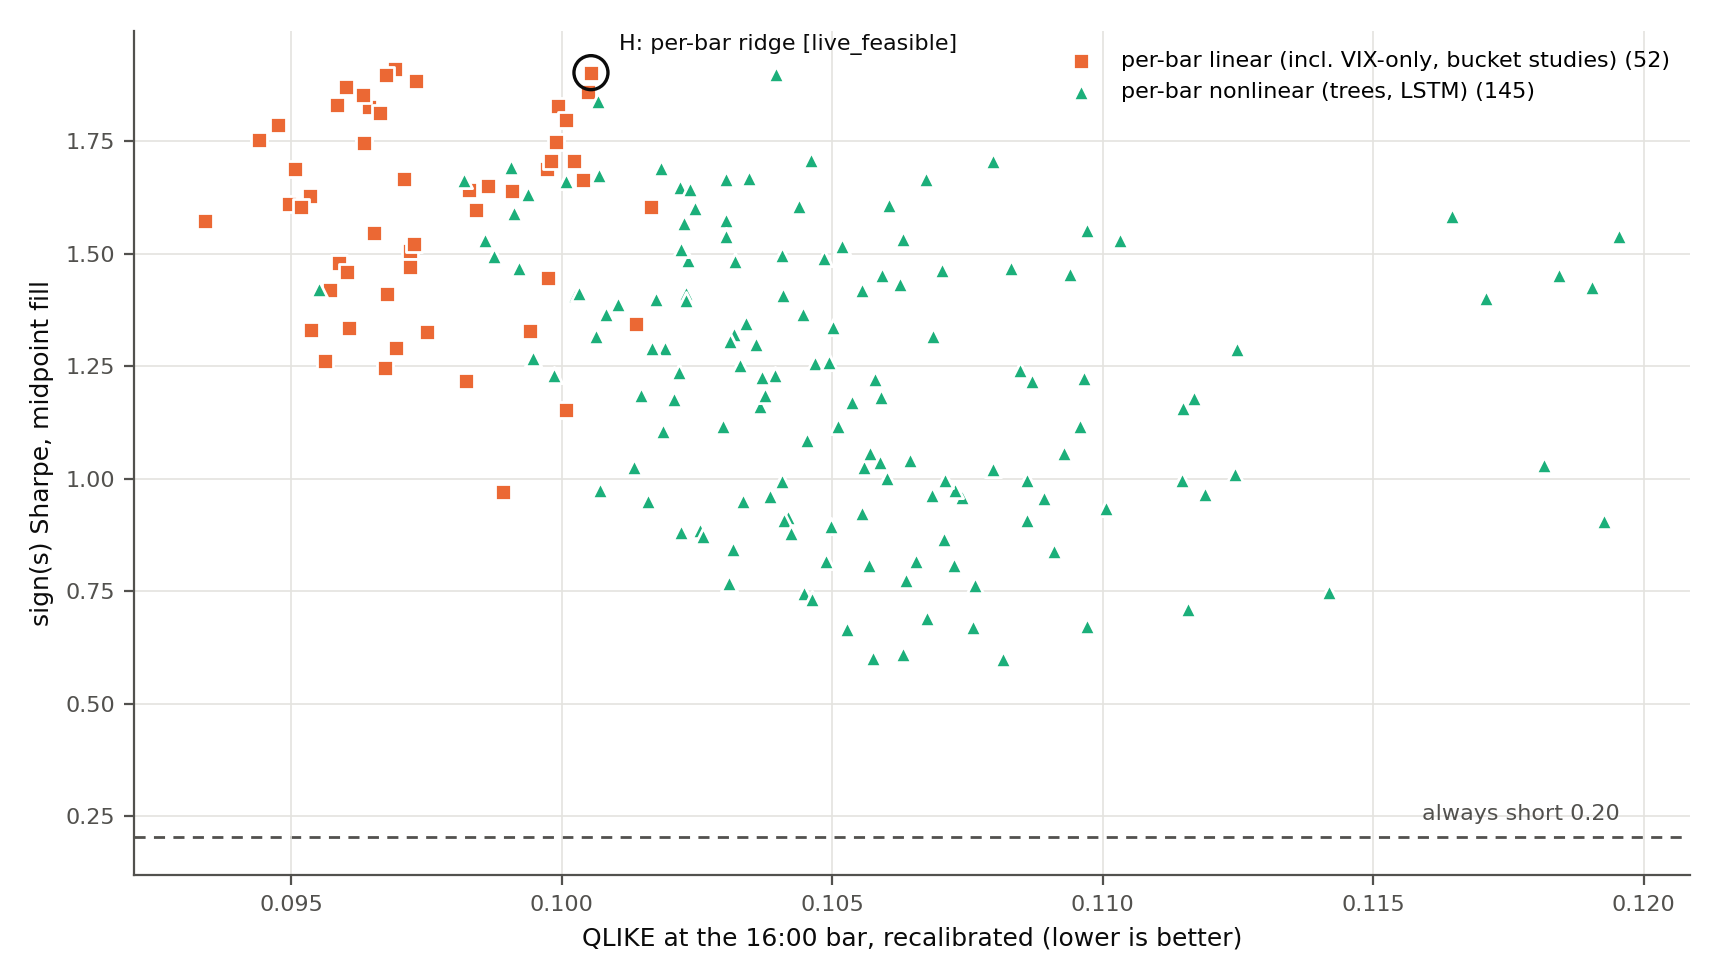
\includegraphics[width=0.85\linewidth]{../results/close_master_table/qlike_vs_sharpe_16h.png}
\caption{Recalibrated 16:00 QLIKE against the sign(s) Sharpe ratio (midpoint fill), table A (check rows and identical forecasts left out); the dashed line is always short. R = reference, H = recommended headline. 5 forecasts lie beyond the plotted QLIKE range (upper quartile + 3 interquartile ranges = 0.127) and are not drawn: per-bar LSTM [all\_features] (QLIKE 0.131, Sharpe 1.33); per-bar LSTM, QLIKE-selected [all\_features] (QLIKE 0.130, Sharpe 1.09); per-bar elastic net [live\_feasible], HAR ladder intra (QLIKE 0.214, Sharpe 0.36); per-bar lasso [live\_feasible], HAR ladder intra (QLIKE 0.218, Sharpe 0.19); per-bar ridge [live\_feasible], HAR ladder intra (QLIKE 0.218, Sharpe -0.02).}
\end{figure}
\end{document}
